\documentclass[twocolumn,11pt]{jarticle}

\usepackage[dvipdfmx]{graphicx}
\graphicspath{ {math-images/} }
\usepackage{wrapfig}
\usepackage[dvipdfmx]{color}
\usepackage{geometry}
\usepackage{amsmath}
\usepackage{latexsym}
%\usepackage{ascmac}
\usepackage{fancyhdr}
\usepackage{overpic}
\usepackage[dvipdfmx,%
 bookmarks=true,%
 bookmarksnumbered=true,%
 colorlinks=true,%
 linkcolor=blue,%
 setpagesize=false,%
 pdftitle={数学の基礎訓練I},%
 pdfauthor={西井淳},%
 pdfsubject={数学の基礎訓練},%
 pdfkeywords={数学; 関数}]{hyperref}
\usepackage{pxjahyper}%hyperrefの不具合対応
\usepackage{makeidx} %索引
%\usepackage[extra]{mymath}
\usepackage{mymath}
\makeindex

\newif\ifans
\ansfalse

\geometry{body={178mm,242mm},columnsep=9mm}

\begin{document}

\pagestyle{empty}
\twocolumn[
%\vspace{-0.8cm}
\noindent
\rule{\linewidth}{0.5pt}
\begin{center}
{\Huge\gtfamily 数学の基礎訓練I\\\vspace{0.3cm}
\LARGE〜基本的な概念・関数〜}
\end{center}
%\vspace{-0.6cm}
\begin{flushright}
\today 版\quad 西井 淳
\\
\rule{\linewidth}{0.5pt}
\end{flushright}
]

{\small\tableofcontents}
\newpage
% \rule{0pt}{10cm}
% \newpage

\setcounter{page}{1}
\pagestyle{fancy}

\section{基礎知識}

\subsection{ギリシャ文字}

\noindent
以下の読みを書きなさい
\answer{
(1) $\gamma$:ガンマ~
(2) $\epsilon$:イプシロン~
(3) $\sigma$:シグマ~
(4) $\delta$:デルタ~
(5) $\eta$:イータ~
(6) $\lambda$:ラムダ~
(7) $\rho$:ロー~
(8) $\tau$:タウ~
(9) $\psi$:プサイ~
(10) $\omega$:オメガ~
(11) $\phi$:ファイ~
(12) $\chi$:カイ~
(13) $\mu$:ミュー~
(14) $\xi$:クシー(グザイ)~
(15) $\zeta$:ゼータ~
(16) $\varphi$:ファイ($\phi$の変形)~
(17) $\varepsilon$:イプシロン($\epsilon$の変形)~
(18) $\kappa$:カッパ~
(19) $\nu$:ニュー~
(20) $\Gamma$:ガンマ~
(21) $\Pi$:パイ~ 
(22) $\Sigma$:シグマ~
(23) $\Theta$:シータ~
(24) $\Lambda$:ラムダ~
(25) $\Delta$:デルタ~
(26) $\Phi$:ファイ~
(27) $\Psi$:プサイ 
(28) $\Omega$:オメガ~
}。

\noindent
(1) $\gamma$~
(2) $\epsilon$~
(3) $\sigma$~
(4) $\delta$~
(5) $\eta$~
(6) $\lambda$~
(7) $\rho$~
(8) $\tau$\\
(9) $\psi$~
(10) $\omega$~
(11) $\phi$~ 
(12) $\chi$~
(13) $\mu$~
(14) $\xi$~
(15) $\zeta$\\
(16) $\varphi$
(17) $\varepsilon$
(18) $\kappa$~
(19) $\nu$~
(20) $\Gamma$~ 
(21) $\Pi$~\\
(22) $\Sigma$~
(23) $\Theta$~
(24) $\Lambda$~
(25) $\Delta$~
(26) $\Phi$~
(27) $\Psi$~\\
(28) $\Omega$


%% \subsection{簡単な計算}
%% \begin{enumerate}
%% \item $(x^2 \cdot x^3)^4$
%% \item $\displaystyle\frac{(e^x)^3}{(e^2)^x}$
%% \end{enumerate}

\subsection{数列の和と積}
ギリシァ文字$\Sigma$はアルファベットのSに対応するので,和(Sum)の記
号として使われている\index{$\sum$}。
ギリシァ文字$\Pi$はアルファベットのPに対応するので,積(Product)の記号
として使われている\index{$\prod$}。
以下は例である。
\begin{align}
 \sum_{n=1}^3n^2&=1^2+2^2+3^2=14\notag\\
 \prod_{n=1}^3n^2&=1^2\cdot 2^2\cdot 3^2=36\notag
\end{align}
記号$\sum$や$\prod$の下には変数名とその最小値を, 上には最大値を書く。
上の例では変数$n$の最小値を$1$, 最大値を$3$とする整数の集合
\begin{quote}
  $n\in\{1,\ldots,3\}$
\end{quote}
に対して記号の右にある式の総和や総乗を計算している。
なお, $\sum$や$\prod$で指定した変数のとるべき値が空集合になるときには, 
$\sum$による総和は0, $\prod$による総乗は1とする。

以下は複数の$\sum$を用いた表現の例である。
\begin{align}
 \sum_{j=0}^2&\sum_{k=0}^2(j+k)=\sum_{j=0}^2\left(\sum_{k=0}^2(j+k)\right)\notag\\
 &=\sum_{k=0}^2(0+k)+\sum_{k=0}^2(1+k)+\sum_{k=0}^2(2+k)\notag\\
 &=(0+1+2)+(1+2+3)+(2+3+4)\notag\\
 &=18\notag
\end{align}
上記の計算は次のようにすることもできる。
\begin{align}
 \sum_{j=0}^2&\sum_{k=0}^2(j+k)=\sum_{j=0}^2\left(\sum_{k=0}^2(j+k)\right)\notag\\
 &=\sum_{j=0}^2((j+0)+(j+1)+(j+2))\notag\\
 &=\sum_{j=0}^23(j+1)\notag\\
 &=3((0+1)+(1+1)+(2+1))\notag\\
 &=18\notag
\end{align}

\nquestion
以下を計算しなさい
\answer{
(\ref{item:sum_n=(1-3)n+1}) 7~
(\ref{item:sum_n=(1-3)(n+1)}) 9~
(\ref{item:nosum}) 0~
(\ref{item:noprod}) 1~
(\ref{item:sum_n=(1-3)1}) 3~
(\ref{item:prod_n=(1-3)2}) 8~
(\ref{item:sum(-)^n}) $-3$~
(\ref{item:prod_n=(2-5)(n+2)/n}) 7~
(\ref{item:sum_j=(0-2)sum_k=(0-j)(j+k)}) 12~
% (\ref{item:sum_n=(1-3)prod_(k=(0-2)(n+k)}) 90~
% (\ref{item:sum_k=(0-2)prod_l=(1-k)l^k}) 5~
(\ref{item:sum_k=(0-2)prod_l=(1-k)2^l}) 11~
}。
\begin{enumerate}
\item\label{item:sum_n=(1-3)n+1} $\displaystyle\sum_{n=1}^3n+1$
\item\label{item:sum_n=(1-3)(n+1)} $\displaystyle\sum_{n=1}^3(n+1)$
\item\label{item:nosum} $\displaystyle\sum_{n=1}^0n$
\item\label{item:noprod}$\displaystyle\prod_{k=3}^0k$
\item\label{item:sum_n=(1-3)1} $\displaystyle\sum_{n=1}^31$
\item\label{item:prod_n=(1-3)2} $\displaystyle\prod_{n=1}^32$
\item\label{item:sum(-)^n} $\displaystyle\sum_{n=0}^5 (-)^n n$
% \item\label{item:sum_n=(1-3)n(n+1)/2} $\displaystyle\sum_{n=1}^3\frac{n(n+1)}{2}$
\item\label{item:prod_n=(2-5)(n+2)/n} $\displaystyle\prod_{n=2}^{5} \frac{n+2}{n}$
 \item\label{item:sum_j=(0-2)sum_k=(0-j)(j+k)} $\displaystyle\sum_{j=0}^2\sum_{k=0}^j(j+k)$
% \item\label{item:sum_n=(1-3)prod_(k=(0-2)(n+k)}$\displaystyle\sum_{n=1}^{3} \prod_{k=0}^{2}(n+k)$
% \item\label{item:sum_k=(0-2)prod_l=(1-k)l^k}$\displaystyle\sum_{k=0}^{2} \prod_{l=1}^{k}l^k$
\item\label{item:sum_k=(0-2)prod_l=(1-k)2^l}$\displaystyle\sum_{k=0}^{2} \prod_{l=1}^{k}2^l$
\end{enumerate}

\nquestion
以下の各数列の第$n$項までの和をそれぞれ$\sum$を一つだけ用いて表しなさい
\answer{
% (\ref{item:1+2+3})~ $\displaystyle\sum_{k=1}^nk$
% (\ref{item:2+4+6})~ $\displaystyle\sum_{k=1}^n(2k)$
(\ref{item:1+3+5})~ $\displaystyle\sum_{k=1}^n(2k-1)$~
(\ref{item:1-2+3-4})~ $\displaystyle\sum_{k=1}^n(-)^{k-1}k$~
% (\ref{item:1+2x1+3x2x1})~ $\displaystyle\sum_{k=1}^nk!$
(\ref{item:2x1+3x2})~ $\displaystyle\sum_{k=1}^n(k+1)k$
}。
\begin{enumerate}
% \item\label{item:1+2+3} $\displaystyle 1+2+3+4+5+\cdots$
% \item\label{item:2+4+6} $\displaystyle 2+4+6+8+10+\cdots$
\item\label{item:1+3+5} $\displaystyle 1+3+5+7+9+\cdots$
\item\label{item:1-2+3-4} $\displaystyle 1-2+3-4+5-6+7-8+9-\cdots$
  % \item $\displaystyle 1+2-3-4+5+6-7-8+9+10-\cdots$
% \item\label{item:1+2x1+3x2x1} $\displaystyle 1+2\times 1 + 3\times 2\times 1+ 4\times 3\times
%   2\times 1+\cdots$
\item\label{item:2x1+3x2} $\displaystyle 2\times 1 + 3\times 2+ 4\times 3 +\cdots$
\end{enumerate}

%%%%%%
\nquestion
以下の空欄に適切な数式を記入しなさい
\answer{(1) $k-t$~ (2) $i+t+1$~ (3) $T-i-1$}。
\begin{align}
  r_{t+1}&+\gamma r_{t+2}+\gamma^2 r_{t+3}+\cdots+\gamma^{T-1}r_{t+T}\notag\\
  &=\sum_{k=t}^{T+t-1}\gamma^{\snbox{(1)}}r_{k+1}\notag\\
  & =\sum_{i=0}^{T-1}\gamma^ir_{\snbox{(2)}}\notag\\
  & =\sum_{i=0}^{T-1}\gamma^{\snbox{(3)}}r_{T+t-i}\notag
\end{align}

%%%%%%
\nquestion
以下のうち等式として成り立つものに◯を, 成り立たないものはには×を記し
なさい。
\begin{enumerate}
\item $\displaystyle\sum_{n=1}^N2n=2\sum_{n=1}^Nn$
%  \quad(答)\nullbox[◯]
\item $\displaystyle\prod_{n=1}^N2n=2\prod_{n=1}^Nn$
%  \quad(答)\nullbox[×]
\item
  $\displaystyle\sum_{i=1}^N\sum_{j=1}^Mf(i,j)=\sum_{j=1}^M\sum_{i=1}^Nf(i,j)$
%  \quad(答)\nullbox[◯]
\item $\prod_{i=1}^N\prod_{j=1}^Mf(i,j)=\prod_{j=1}^M\prod_{i=1}^N(f(i,j)$
\end{enumerate}


\subsection{階乗}
自然数$n$に対して\bfindex[かいじょう]{階乗}(\nmindex{factorial})
は次のように定義される。
\begin{align}
  n!=\prod_{k=1}^nk=n(n-1)\cdots2\cdot 1\notag
\end{align}
ただし,便宜上
\begin{align}
  0!=1\notag  
\end{align}
と定義されていることに注意。
これは
\begin{align}
n!=n\cdot(n-1)!\notag
\end{align}
が$n\ge 1$について成り立つようにするための定義である。

\nquestion
以下を計算しなさい
\answer{
(\ref{item:sum_n=(0-2)n!}) 4~
(\ref{item:prod_n=(0-2)n!}) 2~
(\ref{item:sum_n=(0-3)(n+2)!/n!}) 40~
}
\begin{enumerate}
\item\label{item:sum_n=(0-2)n!} $\displaystyle\sum_{n=0}^2n!$
\item\label{item:prod_n=(0-2)n!} $\displaystyle\prod_{n=0}^2n!$
\item\label{item:sum_n=(0-3)(n+2)!/n!} $\displaystyle\sum_{n=0}^3\frac{(n+2)!}{n!}$
\end{enumerate}

\subsection{幾何学の基礎}

\subsubsection{内角の和}

\nmindex[ゆーくりっどきかがく]{ユークリッド幾何学}
\footnote{ユークリッド幾何学とは古代ギリシアの数学者, 
天文学者であるエウクレイデス(\nmindex{Eukleides}, 
英語名はユークリッド\nmindex{Euclid}, BC365? - BC275?)による
著書「ユークリッド原論」に基づく幾何学。
ただし,エウクレイデスは実在せず「ユークリッド原論」は
共同執筆であるとする説もある。
}
においては\nmindex[こうじゅん]{公準}(仮定)により,
平行線の2つの\bfindex[さっかく]{錯角}は等しい。
\begin{enumerate}
\item 三角形の内角の和が$\pi$であることを証明せよ。
\item 四角形の内角の和はいくつになるかを求めよ。
\item 直径の円周角は直角であることを証明せよ。
\end{enumerate}

\subsubsection{面積}
2辺の長さを$a$, $b$とする長方形が与えられたとき,その
\bfindex[めんせき]{面積}を$ab$で表す。
\begin{enumerate}
\item 底辺の長さと高さが互いに等しい2つの平行四辺形の面積が互いに等し
  いことを幾何学的に証明せよ(図\ref{fig:parallelogram})。
  また,この結果をもとに平行四辺形の面積が「底辺の長さ×高さ」で求まる理
  由を説明せよ。
\begin{figure}[t]
  \begin{center}
    \resizebox{5cm}{!}{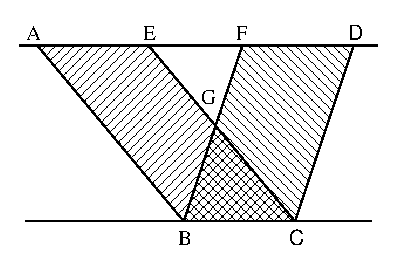
\includegraphics{math-images/parallelogram.eps} }
    \caption{底面の長さと高さが互いに等しい平行四辺形の面積は等しい}
    \label{fig:parallelogram}
  \end{center}
\end{figure}
\item 三角形の面積が「底辺の長さ×高さ÷2」で求まる理由を説明せよ。
%% \begin{figure}[h]
%%   \begin{center}
%%     \resizebox{4cm}{!}{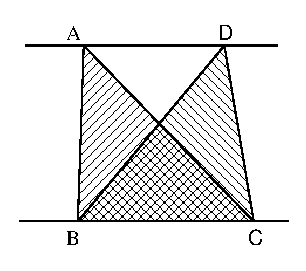
\includegraphics{math-images/triangle.eps} }
%%     \caption{三角形の面積}
%%     \label{fig:triangle}
%%   \end{center}
%% \end{figure}
\end{enumerate}

\subsubsection{三平方の定理}
\nmindex[さんへいほうのていり]{三平方の定理}
(ピタゴラス
\footnote{\nmindex{ピタゴラス}(\nmindex{Pythagoras}, BC582-BC496)
  古代ギリシャの数学者であり哲学者} 
の定理\index{ぴたごらすのていり@ピタゴラスの定理})を証明しなさい。

\subsubsection{三次元空間内の二点間の距離}
三次元空間の$xyz$直交座標系において,点$P(x_1,y_1,z_1)$と点
$Q(x_2,y_2,z_2)$の間の\bfindex[きょり]{距離}(\nmindex{distance})
$PQ$が
\begin{align}
 PQ=\sqrt{(x_1-x_2)^2+(y_1-y_2)^2+(z_1-z_2)^2} \notag
\end{align}
で表されることを証明せよ。

\comment
幾何学的な問題では必ず図を描き,
図でも文でも読み手に伝わるような説明を心がけること。

\subsection{多項式・関数・方程式}

\subsubsection{関数とは}
\bfindex[かんすう]{関数}(\nmindex{function})とは, 
\textbf{入力値を出力値に対応付ける規則}のことである。
つまり, 入力$x$を出力$y$に対応付ける規則$f$が与えられたとき,
\begin{align}
  y=f(x)\quad or\quad x \overset{f}{\longmapsto} y\notag
\end{align}
と書き,この規則のことを関数$y=f(x)$, もしくは関数$f(x)$と呼ぶ。
このとき, $y$を$x$の$f$による\bfindex[ぞう]{像}(\nmindex{image})と呼ぶ。
また,入力値を表す変数$x$を\bfindex[どくりつへんすう]{独立変数}, 
出力値を表す変数$y$を\bfindex[じゅうぞくへんすう]{従属変数}と呼ぶ。


\subsubsection{多項式とは}
\textbf{変数と定数の和と積のみからなる式}を
\bfindex[たこうしき]{多項式}(\nmindex{polynomial})とよぶ。
例えば, 以下の式$f(x)$は変数$x$と定数$a_0,\ldots,a_n$からなる多項式である。
\begin{align}
  \label{eq:polynominal}
  f(x)=a_nx^n+a_{n-1}x^{n-1}+\cdots+a_1x+a_0
\end{align}
% 上式の各項のうち, 次数(じすう, degree)最高次係数

\subsubsection{因数分解}
式(\ref{eq:polynominal})で表される多項式$f(x)$を
\begin{align}
f(x)=(x-c)(b_{n-1}x^{n-1}+\cdots+b_1x+b_0) \notag
\end{align}
と書き直せるとき,
\begin{quote}
$f(x)$は\bfindex[いんすう]{因数}(\nmindex{factor})
$x-c$をもつ
\end{quote}
という。
このようにある多項式をいくつかの多項式の
積で表すことを\bfindex[いんすうぶんかい]{因数分解}
  (\nmindex{factorization})という。
多項式$f(x)$が$x-c$を因数に持つとき次式が成りたつ。
\begin{align}
  f(c)=0  \notag
\end{align}

\nquestion
以下を実数の範囲内で因数分解しなさい。
\begin{enumerate}
\item $x^3-1$
% \item $x^4-1$
\item $x^3+3x^2+4x+2$
% \item $x^2-y^2$
\item $x^n-1$
\end{enumerate}

\nquestion 以下を因数分解しなさい。
因数がすぐにわからないときには, 次数の低い項でまとめると見通しが
  よくなることが多い。
\begin{enumerate}
\item $x^2-2xy-x+2y$
\item $xy^2+3ay^2-a^2x-3a^3$
\end{enumerate}

\subsubsection{関数とグラフ}
% 関数を可視化するには, 入力値(独立変数)を横軸に, 出力値(従属変数)を
% 縦軸にしたグラフを書くことが多い。

\nquestion
以下の各式が表すグラフを2次元$xy$平面に描きなさい。
\begin{enumerate}
\item $y=-2x+1$
\item $y=x^2-x$
% \item $y=x^2-2x+2$
% \item $x^2+y^2-2x=0$
\item $x=1$
\item $x=1$と$y=1$の交わり
\item $x^2+y^2=1$
\end{enumerate}

\comment
グラフを描くときには以下に気をつけること。
\begin{enumerate}
\item 座標軸について
  \begin{enumerate}
  \item 各軸の名前$(x,y)$を書いているか?
  \item 軸の正の向きを矢印で示しているか?
  \item 原点(Origin)を明記しているか?
  \end{enumerate}
\item グラフについて
  \begin{enumerate}
  \item 直線や二次式を描くときは直線の方程式を一意に特定できる情報を記す。
  \item さらに複雑な関数でもその特徴を示す点の情報を記す。
  \end{enumerate}
\end{enumerate}

\nquestion
各式が表すグラフを3次元$xyz$直交座標系に描きなさい。
\begin{enumerate}
\item $x=1$
\item $x=1$と$y=1$の交わり
\item $x^2+y^2+z^2=1$
\item $x^2+y^2+z^2-2y=1$
\item $x^2+y^2=1$
\end{enumerate}

\comment
3次元グラフを描くとき, $x$, $y$軸の向きが決まれば$z$軸の向きが決まるこ
とに注意せよ。

\nquestion
$x^2+y^2=z^2$について以下の問に答えなさい。
\begin{enumerate}
\item $z=0$に対する断面の形を調べて$xyz$直交座標系に図示しなさい。
\item $z=1$における断面の形を調べて上の同じグラフ図示しなさい。
\item $z=2$における断面の形を調べて上の同じグラフ図示しなさい。
\item $x=0$に対する断面の形を調べて$xyz$直交座標系に図示しなさい。
\item 与式はどのような立体図形を表しているか。
\end{enumerate}

\nquestion
関数$y=x^2+2x$について以下の問に答えなさい。
\begin{enumerate}
\item $x\in[0,1]$における最大値と最小値は?
\item $x\in[-2,0]$における最大値と最小値は?
\end{enumerate}

%%%%%%%%%%%
% \begin{extra}
% \nquestion
% 次式で表される領域を図示せよ。
% \begin{enumerate}
% \item $\displaystyle y\ge -2x+1$
% \item $(x^2+y^2-4)(x-y-1)<0$
% \end{enumerate}
% \end{extra}

% \begin{extra}
% \subsubsection{方程式と不等式}
% \nquestion
% 以下の\nmindex[にじほうていしき]{二次方程式}
% (\nmindex{quadratic equation})
% の解を求めなさい。
% ただし解の公式は使わないこと。
% \begin{enumerate}
% \item $ax^2+bx+c=0$, ($a\ne 0$)
% \item $ax^2+2bx+c=0$, ($a\ne 0$)
% \item $x^2+3x+2=0$
% \item $x^2+2x+2=0$
% \end{enumerate}
% \end{extra}
%%%%%%%%%%%%%%%%%%%%%%%%

\subsubsection{方程式とは}

\bfindex[ほうていしき]{方程式}(\nmindex{equation}
\footnote{equationの''equ''は''等しい''という意味の接頭語})とは
\textbf{変数がある値をとるときに両辺が等しくなる等式}のことである。
よって, \textbf{方程式には必ず等号が一つ含まれる。}
また,方程式に含まれる変数はしばしば\textbf{未知数}と呼ばれる。

\nquestion
ここまでに述べた関数と方程式の定義に従い,以下のうち適切でない
表現を選びなさい
\answer{
(1) ×
(2) ○
(3) ×
(4) ×
(5) ○
(6) ×
(7) ○
(8) ○
(9) ×
}
。
\begin{enumerate}
\item 方程式$x^2+1$
\item 方程式$x^2+1=0$
\item 関数$x^2+1=0$
\item 方程式$f(x)$
\item 関数$f(x)$
\item 方程式$y=x^2+1$ ($x$は独立変数。$y$は従属変数)
\item 関数$y=x^2+1$ ($x$は独立変数。$y$は従属変数)
\item 方程式$y=x^2+1$ ($x$も$y$も未知数)
\item 関数$y=x^2+1$ ($x$も$y$も未知数)
\end{enumerate}

\nquestion
以下の問いに答えなさい
\begin{enumerate}
\item $x=1$と$x=2$を解に持ち,$x$の最高次の係数が2である2次方程式を書
  きなさい。
\item $x=1$のみを解に持ち,$x$の最高次の係数が1である2次方程式を書きな
  さい。
\item $x=a$, $x=b$, $x=c$を解に持ち,$x$の最高次の係数が1である
  3次方程式を書きなさい。
\end{enumerate}

%%%%%%
\subsubsection{方程式とグラフ}

方程式$f(x)=g(x)$の解の意味を幾何学的に考えると,
\begin{align}
  \begin{cases}
    y=f(x)\\
    y=g(x)
  \end{cases}\notag
\end{align}
の2曲線の交わりの$x$座標を表す。
このように, 方程式の解は一般にいくつかの直線や曲線,曲面等の交わりと捉
える事もできる。

例えば次式を考えてみよう。
\begin{align}
  2x=1
  \label{eq:2x=1}
\end{align}
上式の解は以下の2直線の交点の$x$座標の値となる(図\ref{fig:2x=1})。
\begin{align}
  \begin{cases}
    y=2x\\
    y=1
  \end{cases}\notag
\end{align}
すなわち,これは以下の2直線の交点として表現できる。
\begin{figure}[tb]
  \centering
  \begin{overpic}[width=6cm]{math-images/axis-tics-2xEq1.eps}
    {
      \put(63,57){解$x=\frac{1}{2}$}
      \put(64,93){$y=2x$}
      \put(96,63){$y=1$}
    }
  \end{overpic}
  \caption{方程式$2x=1$の幾何学的意味\label{fig:2x=1}}
\end{figure}

また,式(\ref{eq:2x=1})を変形して
\begin{align}
  -2x+1=0 \label{eq:-2x+1=0}
\end{align}
と書けば次の2直線の交点の$x$座標と考えることもできる。
\begin{align}
  \begin{cases}
    y=-2x+1\\
    y=0
  \end{cases}\notag
\end{align}
式(\ref{eq:2x=1})と式(\ref{eq:-2x+1=0})は等価であるが,
幾何学的には異なった意味を持つ。

\nquestion
以下の方程式の解を求めなさい。また, 解の幾何学的意味を説明しなさい。
求めた解は元の方程式に代入する事により,その解が正しいかどうかを確かめ
なさい。
\begin{enumerate}
\item $x^2-x=0$
\item $x^2=x$
\item $x=\sqrt{x}$
\item $x^2-1=0$
\item $\displaystyle x=\frac{1}{x}$
% \item $x^2-3x+2=0$
% \item $\displaystyle\frac{2}{x}=-x+3$
 \item $x^3-3x^2+2x=0$
\item $
  \begin{cases}
    y=x\\
    x^2+y^2=1
  \end{cases}
$
\end{enumerate}

%%%%%%
\nquestion
次の2曲線について以下の問に答えなさい。
\begin{align}
  \begin{cases}
    y&=x^2+2x+1\notag\\
    y&=x+c\notag
  \end{cases}
\end{align}
\begin{enumerate}
\item 2曲線が交点をもつとき,その座標は以下の方程式を解くことにより
  求めることができる。
  \begin{align}
    x^2+2x+1=x+c\notag
  \end{align}
  上式の解はどのような点かをグラフにより示しなさい。
\item 上式を変形すると以下のようになる。
  \begin{align}
    x^2+x+1-c=0\notag
  \end{align}
  上式の解はどのような点かをグラフにより示しなさい。
\item 以下の条件について,(i) (2)のグラフを書いて幾何学的に考える方法,(ii)判別式を用いる方法, (iii)交点を求めるための方程式を因数分解した形に着目した方法でそれぞれ述べなさい。
  \begin{enumerate}
  \item 2曲線が異なる2点で交わる。
  \item 2曲線が接する。
  \item 2曲線が交点を持たない。
  \end{enumerate}
\end{enumerate}

%%%%%%
\nquestion
2曲線$y=x^2+c$と$x^2+y^2=1$について以下の問いに答えなさい。
\begin{enumerate}
\item $c=1$のとき2曲線の接点や交点の数を答えなさい。
また, 各接点や交点の$x$座標を解とする方程式を因数分解した形を答えなさい。
\item $c=-1$のとき2曲線の接点や交点の数を答えなさい。
また, 各接点や交点の$x$座標を解とする方程式を因数分解した形を答えなさい。
\item 2曲線の交点や接点の数が$c$の値によってどう変わるか,またその時
  $x$座標を解とする方程式を因数分解した形がどう変わるかを答えなさい。
\end{enumerate}

%%%%%%%%%%%%
\subsubsection{不等式とグラフ}
\bfindex[ふとうしき]{不等式}(\nmindex{inequality})とは
\textbf{不等号を含んだ式}であり, 二つの式の大小を評価するためのもので
ある。

以下の不等式の幾何学的意味を考えてみよう。
\begin{align}
f(x)> g(x)\qquad\cdots(*)\notag
\end{align}
上式の左辺および右辺によって与えられる以下の2式がつくる2曲線を
それぞれ$l$, $m$とする。
\begin{align}
  \begin{cases}
    l: y=f(x)\\
    m: y=g(x)
  \end{cases}\notag
\end{align}
不等式(*)の解は, 曲線$l$の$y$の値が曲線$m$に比べて大きくなるような
$x$の範囲を意味する。

例えば, $2x>1$の解は
\begin{align}
  \begin{cases}
    y=2x\\
    y=1
  \end{cases}\notag
\end{align}
の2直線のうち前者の値$y$のほうが大きくなるような$x$の範囲を意味する
(図\ref{fig:ineq})。
\begin{figure}[t]
  \centering
  \begin{overpic}[width=6cm]{math-images/axis-tics-2xIneq1.eps}
    {
      \put(67,75){解$x>\frac{1}{2}$}
      \put(64,93){$y=2x$}
      \put(96,63){$y=1$}
    }
  \end{overpic}
\caption{不等式$2x>1$の幾何学的表現\label{fig:ineq}}
\end{figure}

\nquestion
以下の不等式の解を求めなさい。また, 2次元$xy$空間における解の幾何学的
意味を説明しなさい。
また,求めた解をみたすいくつかの値を$x$に代入する事により,その解が正
しいかどうかを確かめなさい。
\begin{enumerate}
\item $2x\ge 1$
\item $x^2-x> 0$
\item $x^2>x$
\item $x>\sqrt{x}$
\item $x^2-1\le 0$
\item $\displaystyle x>\frac{1}{x}$
% \item $x^2-3x+2<0$
% \item $\displaystyle\frac{2}{x}\ge -x+3$
\item $x^3-3x^2+2x<0$
\end{enumerate}

\nquestion
以下の問に答えなさい
\answer{
(\ref{item:2(x-1)(x-2)>0}) $2(x-1)(x-2)>0$~
(\ref{item:(x-1)^2<=0}) $(x-1)^2\le 0$~
(\ref{item:(x-a)(x-b)(x-c)<0}) $(x-a)(x-b)(x-c)< 0$
}
\begin{enumerate}
\item\label{item:2(x-1)(x-2)>0} 
  $x<1$と$2<x$を解に持ち,$x$の最高次の係数が2である
  2次不等式を書きなさい。
\item\label{item:(x-1)^2<=0} 
  $x=1$のみを解に持ち,$x$の最高次の係数が1である
  2次不等式を書きなさい。
\item\label{item:(x-a)(x-b)(x-c)<0} 
  $a<b<c$とするとき,
  $x<a$, $b<x<c$を解に持ち,$x$の最高次の係数が1である
  3次不等式を書きなさい。
\end{enumerate}
\subsubsection{合成関数}

入力値$x$に対して関数$f$で変換した後, さらに関数$g$で変換して得られる
出力を$y$とするとき, この演算は次のように書く。
\begin{align}
  y=g(f(x))\quad \mbox{or}\quad y=(g\circ f)(x)\notag
\end{align}
\nquestion
$f(x)=2x$, $g(x)=x+1$とするとき, 下記の問に答えなさい
\answer{
$(f\circ g)(x)=f(g(x))=f(x+1)=2(x+1)$,\quad
$(g\circ f)(x)=g(f(x))=g(2x)=2x+1$\quad
(\ref{item:fg2}) $(f\circ g)(2)=6$\quad
(\ref{item:gf2}) $(g\circ f)(2)=5$
}。
\begin{enumerate}
\item\label{item:fg2} $(f\circ g)(2)$の値は?
\item\label{item:gf2} $(g\circ f)(2)$の値は?
\end{enumerate}

\nquestion
$f(x)=g(x^2)-1$, $g(x)=x+1$のとき, 
$f(g(x))=g(f(x))$となる$x$を求めなさい
\answer{
$f(g(x))=f(x+1)=(x+1)^2$,\;\;
$g(f(x))=g(g(x^2)-1)=g((x^2+1)-1)=x^2+1$
より両者が等しくなる$x$は$x=0$。
}。

\subsubsection{二次曲線}

$x$, $y$に関する二次方程式で表される曲線を二次曲線という。
2次元$xy$平面においてその方程式を一般的に書くと以下のようになる。
\begin{align}
  ax^2+by^2+pxy+qx+ry+c=0\quad(a,b,p,q,c\mbox{:定数})\notag
\end{align}
その典型的な形は以下のように分類される。
\begin{enumerate}
\item 放物線: $y=ax^2$, $x=ay^2$ 
\item 円, 楕円: $ax^2+by^2=c$ ($a,b,c>0$)
\item 双曲線: $ax^2-by^2=c$
\end{enumerate}

各図形の幾何学的意味は以下のとおりである。
\begin{enumerate}
\item 放物線とは平面上のある点と, その点を通らない直線からの距離が等し
  い点の集合である。
\item 円とは平面上のある点から等しい距離にある点の集合である。
\item 楕円とは平面上のある二点からの距離の和が一定である点の集合である。
\item 双曲線とは平面上のある二点からの距離の差が一定である点の集合である。
\end{enumerate}

\nquestion
以下の\textbf{定性的表現}を表すグラフ(\textbf{幾何学的表現})を描きなさ
い。
また\textbf{定量的表現}としてできるだけ簡単な数式で表しなさい
\answer{
  (\ref{jitem:circle}) $\sqrt{(x-2)^2+(y-2)^2}=2$~
  (\ref{jitem:ellipse}) $\frac{x^2}{4}+\frac{y^2}{3}=1$
  (\ref{jitem:parabola}) $y=\frac{1}{2}(x-1)^2+\frac{1}{2}$
  (\ref{jitem:sphere}) $\sqrt{(x-a)^2+(y-b)^2+(z-c)^2}=1$~
}。
\begin{enumerate}
\item\label{jitem:circle} 平面上で点($2,2$)から距離2の点の集合。
\item\label{jitem:ellipse} 
  平面上で点($1,0$)と点($-1,0$)からの距離の和が4の点の集合。
\item\label{jitem:parabola} 平面上で点($1,1$)と$x$軸から等距離にある
  点の集合。
\item\label{jitem:sphere} 3次元空間内で点($a,b,c$)から距離1の点の集合。
\end{enumerate}


%%%%%
\subsection{基礎的な関数の応用例}
\subsubsection{最適化問題}
ある関数$f(x)$が最大もしくは最小となる$x$を求めることを
\bfindex[さいてきかもんだい]{最適化問題}(\nmindex{optimization problem})とよび,この関数$f$を\bfindex[もくてきかんすう]{目的関数}(\nmindex{objective function} or \nmindex{cost function})とよぶ。
また,$x$がなんらかの条件$g(x)=0$を満たさないといけない時,この条件を\bfindex[せいやくじょうけん]{制約条件}(\nmindex{constraint function})とよぶ。

最適化関数は物理学ではエネルギーを表す関数と対応する。最適化問題は物理計算,機械学習などの情報科学,経営手法を議論する経済学等幅広い分野で扱われる。
最適化問題の解法は目的関数や制約条件によって様々な方法が提案されているが,解析的に解くよりも幾何学的に考えた方が簡単に解けることも多い。

%%%%%%
\nquestion
以下の問に答えなさい
\answer{
(\ref{item:range(x+y)})(a)~
	目的関数は$z=x+y$, 制約条件は$x^2+y^2=4$。
(\ref{item:range(x+y)})(b)~最適解は$(x,y)=(\sqrt{2},\sqrt{2})$, この時の目的関数の値は$2\sqrt{2}$~
(\ref{item:min(x^2+y^2)})~$\min(x^2+y^2)=1/2$, $(x,y)=(1/2,1/2)$
}。
\begin{enumerate}
\item\label{item:range(x+y)} $x^2+y^2=4$の条件下において,$x+y$の最大値を求めたい。
	\begin{enumerate}
	\item 目的関数と制約条件が何か説明しなさい。
	\item $xy$平面上に目的関数と制約関数を図示し,最適解を求めなさい,また,$x$, $y$が最適解となる時の目的関数の値を求めなさい。
	\end{enumerate}
\item\label{item:min(x^2+y^2)} $x+y=1$の条件下において,$x^2+y^2$の最小値と,そのときの$x$, $y$の値を述べなさい。
\end{enumerate}

%%%%%%
\nquestion
杢兵衛商会(もくべえしょうかい)では木工製品の製造販売をしている。
社長の杢兵衛さんは利益を上げるための分析をしたところ以下が判明した。
机を一つ作るのに必要な材料は板1枚であり, 製作時間は5時間, その儲けは
4000円である。
本棚を一つ作るのに必要な材料は板1枚と角材1本であり, 製作時間は1時間, 
その儲けは1000円である。
1週間あたりに, 机と本棚の製造に使える時間は34時間であり, 板は10枚まで, 
角材は6本までである。
\begin{enumerate}
\item 1週間あたりに製造する机と本棚の数をそれぞれ$x$と$y$とする。
杢兵衛さんの目的は1週間あたりの総もうけ額$r$を最大にすることである。
目的関数と,$x$, $y$に関する制約条件を全て数式にしなさい
\answer{
(答)
\begin{align}
制約条件は
  \begin{cases}
  1 \mbox{枚/台} x+ 1\mbox{枚/台} y&\le 10 [枚]\\
  1 \mbox{本/台} y&\le 6 [本]\\
  5 \mbox{hr/台} x+y \mbox{hr/台}&\le 34 \mbox{[hr]}\\
  \end{cases}\notag
\end{align}
目的関数は
\begin{align*}
  r&=4000\mbox{[円/台]} x+1000 \mbox{円/台} y
\end{align*}
問題文に明記されていない以下の暗黙の条件もある。
\begin{align}
  \begin{cases}
  0&\le x\\
  0&\le y
  \end{cases}\notag
\end{align}
}。
\item 1週間あたりの総もうけ額を最大にするには, 机と本棚の
  毎週の製造台数をそれぞれいくつにすればよいか
  \answer{(答)机を6台, 本棚を4台にするとよい。
    (ヒント)上の不等式をみたす$x,y$の領域をグラフに明示す
    る。その領域と目的関数が交わる範囲内で
    $r$を様々に変え,その中で$r$が最大となる点を見つける。}。
\end{enumerate}

%%%%%
\subsubsection{脳の学習理論}

脳の基本素子である神経細胞は,互いに結合しあってネットワーク状の構造を形成している。
神経細胞の出力信号は0, 1で表現できるインパルス状の信号であり,また,
他の神経細胞からの入力に強く活性化された時に出力信号が得られる。
生理学者McCullochと数学者Pittsは,このような生理学的知見に基づいて,1943年に神経細胞の特性を
以下のように数理モデル化した。

\begin{wrapfigure}[5]{r}{4.5cm}\vspace{-.8cm}
  \begin{center}
    \begin{overpic}[width=4cm]{perceptron.eps}
      \put(-10,30){\Large$x_1$}
      \put(-10,7){\Large$x_2$}
      \put(20,38){\Large$w_1$}
      \put(20,16){\Large$w_2$}
      \put(60,16){\Large$\theta$}
      \put(100,20){\Large$z$}
    \end{overpic}\\
    図
  \end{center}
\end{wrapfigure}
ここでは,簡単のため神経細胞が2入力のみを受け取るとする(右図)。
神経細胞が出力信号を出している状態を$z=1$, 出していない状態を$z=0$で表すと,
入力$(x_1,x_2)$と出力$z$は以下の関係式で表現される。
\begin{align*}
  z=\begin{cases}    
    1 & \text{($w_1x_1+w_2x_2\ge\theta$ のとき)}\\
    0 & \text{($w_1x_1+w_2x_2<\theta$ のとき)}
  \end{cases}
\end{align*}
ここで,$w_1$, $w_2$は各入力信号が神経細胞に及ぼす影響を表す定数(結合重み)を, $\theta$は神経細胞の活動のしやすさを表す閾値を表す。

%%%%%
\nquestion
上述の神経回路モデルについて以下の問いに答えなさい。
\begin{enumerate}\label{q:perceptron}
	\item AND回路と同じ入出力関係を実現するには, $(w_1,w_2,\theta)$をどのように選べば良いか。適切な組み合わせを一つ述べなさい
\answer{(答)~$(w_1,w_2,\theta)=(1,1,1.5)$}。
\item
未学習の状態の脳の神経パラメータ($w_1$, $w_2$, $\theta$)はランダムな値となっており,学習とともに少しずつ変化していくと考えられる。
上記の素子に$(x_1,x_2)=(1,0)$を入力したところ$z=0$が出力された。
この時,各パラメータが少しずつ(例えば$0.1$ずつ)変化するとして,どのように増減すれば出力が正解と一致する可能性があるだろうか
\answer{(答) $w_1$:少し大きくする。 $w_2$:変化させても出力に無関係。$\theta$: 少し小さくする。}。
\end{enumerate}
前問のようなアイデアに基づき,Rosenblattは1957年に\nmindex{パーセプトロン}(\nmindex{Perceptron})と呼ばれる脳の学習モデルを発表した。
実際に小脳ではこのような学習が行われていること(小脳パーセプトロン説)がその後の生理学実験で示唆されている。


%%%%%%
\subsection{数式, 定性的表現, 幾何学的表現}

\subsubsection{基本的な表現}
\nquestion
以下の\textbf{定性的表現}をグラフや図形(\textbf{幾何学的表現})を書いて
説明しなさい。
また\textbf{定量的表現}としてできるだけ簡単な数式で表しなさい。
必要に応じて変数の定義をすること。ただし,変数名はできるだけわかりやす
くつけること
\answer{
  (\ref{jitem:linear}) $y=ax+b$ ($a,b$は定数), もしくは $ax+by+c=0$
  ($a,b,c$は定数)
  (\ref{jitem:prop}) $y=kx$ ($k$は比例定数)
  (\ref{jitem:taro}) $E_{taro}<60$ ($E_{taro}$は太郎の英語の点)
  (\ref{jitem:jiro}) $E_{jiro}\le 60$ ($E_{jiro}$は次郎の英語の点)
  (\ref{jitem:sabu}) $E_{sabu}\ge 80$ ($E_{sabu}$は三郎の英語の点)
  (\ref{jitem:Fn}) $F=k/n$ ($F$は力,$n$は単位時間あたりの回転数, $k$は比例定数)
%   (\ref{jitem:VS}) $S=|V|$ ($S$は速さ,$V$は速度)
%   (\ref{jitem:fgsign}) $\forall x\in\Real,\;f(x)g(x)>0$
%  (\ref{jitem:fgsign2}) $\exists x\in\Real,\;f(x)=g(x)$
}。
\begin{enumerate}
\item\label{jitem:linear} 2つの値$x$と$y$が線形関係にある。
\item\label{jitem:prop} 2つの値$x$と$y$が比例関係にある。
\item\label{jitem:taro} 太郎くんの英語の点は60点未満である。
\item\label{jitem:jiro} 次郎くんの英語の点は60点以下である。
\item\label{jitem:sabu} 三郎くんの英語の点は80点以上である。
\item\label{jitem:Fn} 直流モーターの出す力は,単位時間あたり
  の回転数に反比例する。
% \item\label{jitem:VS} 速さ(speed)とは速度(velocity)の大きさである。
% \item\label{jitem:fgsign} 任意の実数$x$に対して, 2つの関数$f(x)$と$g(x)$の符
%   号が同じである。
% \item\label{jitem:fgsign2} ある実数$x$に対して, 関数$f(x)$と$g(x)$は
%    等しい。
\item 時刻$t_1$から時刻$t_2$までの間の,物体の位置$x(t)$の変化が 3 m であった。
\item 時刻$t_1$から時刻$t_2$までの間の,物体の位置$x(t)$の変化を変位$\Delta x$とよぶ。
\end{enumerate}

\subsubsection{和文数訳}
%%%%%%
% \nquestion
% ある店でバットとボールの両方を買うと1100円かかる。
% バットはボールより1000円高かった。
% バットとボールはそれぞれいくらか?

%%%%%%
\nquestion
以下の例題を読んで, その後の問いに答えなさい。

\noindent
[例題]
以下の文章を数式で表しなさい。
\begin{quote}
  現在の花子の年齢は5年前の桜子の年齢の2倍である。
\end{quote}
\noindent
(答)
\begin{quote}
  現在の花子と桜子の年齢を\textbf{それぞれ}$H$, $S$とおく。
  \textbf{題意より次式が成り立つ。}
  \begin{align}
    H=2(S-5)\notag
  \end{align}
\end{quote}
\noindent
(例題の説明)
以下は定式化における注意点。
\begin{enumerate}
\item 頭文字等を利用して\textbf{変数はわかりやすく}定義する。
\item 定式化をするときには, 機械的に文章を式に置き換える。
  \textbf{余計な変形は一切しない}こと。
\item \textbf{説明を文章で}きちんと書く。
\item 答の文中の太字は定型的な言い回し。必ず覚える。
\end{enumerate}

\noindent
[問]
以下の文章を数式で表しなさい。
\begin{quote}
  5年前には, 太郎の年齢は花子の3倍だった。
  10年前には, 太郎の年齢は桜子の半分だった
\answer{
  \textbf{現在の}太郎,桜子,花子の年齢を
  \textbf{それぞれ}$T$,$H$,$S$とおく。
  \textbf{題意より次式が成り立つ}。
  \begin{align}
    \begin{cases}
      T-5 &= 3(H-5)\\
      T-10 &= (S-10)/2
    \end{cases}\notag
  \end{align}
  注) 知りたいのは現在の歳なので, 例えば5年前の年齢を変数にする
  のはミスのもと。また, 変数名はできるだけ誤解がないようにする。
  ここでは太郎たちの頭文字を使った。$x,y,z$等とするとどれが何かわから
  なくなる。
}。
\end{quote}

%%%%%%
\nquestion
以下の例題を読んで, その後の問に答えなさい。

「速度$v$で100 m 移動するのにかかる時間」を数式で表す時には
以下のように書く。
\begin{align}
\frac{100 \mbox{~[m]}}{v}\notag
\end{align}
このように\textbf{数値の単位は必ず明記}する。

一方,以下は悪い例である。
\begin{enumerate}
\item $\displaystyle\frac{100}{v}$
\item $\displaystyle\frac{100\mbox{~[m]}}{v\mbox{~[m$/$s]}}$
\item $\displaystyle\frac{100\mbox{~[m]}}{v}$ [s]
\end{enumerate}
(1)では,$v$が与えられても計算結果が何を表す量かわからなくなる。
$v$の単位は数値とともに与えられれば良いので, (2)のように
$v$単位を事前に決める必要は無いし,
移動にかかる時間は,必要に応じて秒で答えることも時速で答えることも
できるので,(3)のように事前に決める必要も無い。

\noindent
[問]  花子が自転車で15 km走るのにかかる時間は, 6 kmの距離を歩くときにか
かる時間と同じである。花子が自転車で進む速度は, 歩く速度よりも時速9 km
だけ速い。自転車での移動のときも徒歩のときもそれぞれ一定の速度で移動す
るものとする。

上記の問題文を数式にしなさい
\answer{
  \textbf{花子が自転車ですすむ速度と歩く速度}を
  \textbf{それぞれ}$v_b$, $v_w$とする。
  \textbf{題意より次式が成り立つ}。
  \begin{align}
    \begin{cases}
      \frac{15 \mbox{[km]}}{v_b}&=\frac{6 \mbox{[km]}}{v_w}\\
      v_b&=v_w+9 \mbox{[km/hr]}
    \end{cases}\notag
  \end{align}
}。
% \item 花子が歩く速度を求めなさい。\\
%   \aline[時速6km]{7cm}

\exercise
以下の文を,それぞれ1つの数式で表しなさい。
\begin{enumerate}
	\item 太郎の年齢は花子の年齢の半分である。
	\item 太郎と花子の年齢の差は5歳である。
	\item 太郎の年齢は,5年前の花子の年齢の2倍である。
\end{enumerate}


%%%%%%%%%%%%%%%%%%%%%%%%%%%
\subsection{弧度法と度数法}
\subsubsection{角度の定義}

\begin{figure}[h]
  \centering
%  \begin{overpic}[width=4cm,grid,tics=10]{math-images/radian.eps}
  \begin{overpic}[width=4cm]{math-images/radian.eps}
    \put(40,40){$O$}
%    \put(67,54){$\theta$}
    \put(94,42){$x$}
    \put(42,100){$y$}
    \put(57,65){$1$}
    \put(87,42){$1$}
    \put(42,90){$1$}
    \put(0,42){$-1$}
    \put(37,5){$-1$}
    \put(87,62){$\theta$}
%    \put(78,82){$P$}
  \end{overpic}
  \caption{弧度法}
  \label{fig:radian}
\end{figure}
\textbf{弧度法}とは, 
\begin{quote}
  半径1の円において,長さが1である弧を見込む中心角を1\bfindex{ラジアン}
  (\nmindex{radian})[rad]
  \footnote{ラジアン(radian)は半径を表す語radiusと語源は同じ}
\end{quote}
として角度を表す方法のことである(図\ref{fig:radian})。
言いかえると,
扇型の弧長$x$が半径$r$の$\theta$倍であるならば,すなわち
\begin{align}
  x=r\theta \notag
\end{align}
ならば,この比率$\theta$を用いてこの扇型の中心角を表す方法を弧度法とよぶ。
この場合の中心角は
\begin{align}
\theta=\frac{x}{r}\; \mbox{[rad]}\notag
\end{align}
と表されることになる。
\textbf{ラジアンは半径に対する弧長の比}による角度表現なので
本来は\textbf{単位の無い実数}であるが,あえてラジアンという単位をつけ
ることで角度を表すことを示している。

一方,円の中心を通る直線で均等に円周を360分割してできる扇型の中心角
を1度(1$^\circ$もしくは1[deg]と書く)として角度を表す方法を
\textbf{度数法}という。

\bfindex[こくさいたんいけい]{国際単位系}(\bfindex[SIたんいけい]{SI単位系}
\footnote{フランス語で Le Syst\`{e}me International d'Unit\'{e}sの省略
形。英語ではThe International System of Units. 時間[s], 長さ[m], 質量
[kg], 電流[A], 熱力学的温度[K], 物質量[mol], 光度[cd]を基本単位とする
}
)ではラジアンが角度の単位として定められており,
数学・情報・物理分野での角度の表記はラジアンが一般的である。

\begin{enumerate}
%% \item 角度の弧度法による単位「ラジアン(radian)」の定義を述べよ。
\item 度数法による角度$\theta^\circ$を,
  弧度法による値$\theta$ [rad]に変換するための式を述べなさい
\answer{$\theta$ [rad]$=\frac{2\pi}{360^\circ}\theta^\circ$}。
\item 以下は何ラジアンか答えなさい。
  \begin{quote}
    (1) 45$^\circ$\quad
    (2) 360$^\circ$\quad
    (3) 270$^\circ$\\
    (4) 90$^\circ$\quad
    (5) 225$^\circ$\quad
    (6) 180$^\circ$\\
    (7) 120$^\circ$\quad
    (8) 60$^\circ$\quad
    (9) $-30^\circ$\quad
  \end{quote}
\item 1ラジアンは度数法では何度程度か。以下から最も近い値を選びなさい。
  \begin{center}
    (1) $30^\circ$\quad
    (2) $60^\circ$\quad
    (3) $90^\circ$\quad
    (4) $180^\circ$
  \end{center}
\item 以下の円弧の長さを答えなさい
\answer{
(\ref{citem:2m1rad}) 2 m~
(\ref{citem:10cmPIrad}) $10\pi$ cm
(\ref{citem:rtheta}) $r\theta$
}。
  \begin{enumerate}
  \item\label{citem:2m1rad} 半径$2$ m,中心角1 rad の円弧
  \item\label{citem:10cmPIrad} 半径$10$ cm,中心角$\pi$ [rad]の円弧
  \item\label{citem:rtheta} 半径$r$,中心角$\theta$ [rad]の円弧
  \end{enumerate}
\end{enumerate}

\subsubsection{地球の大きさを求める}
\nquestion 以下の問いに答えなさい。
\begin{enumerate}
\item 地球と太陽の間の距離を$R$, 地球の半径を$r$, 太陽の中心から地球を見込む角\footnote{地球全体をちょうど覆える角度}を$\theta$とおく。$r$を$R$と$\theta$を用いて表しなさい。
\item 地球と太陽の間の距離を$R$は季節により若干変化するが, 平均すると
  $R=1.5\times 10^8$ km, 地球の半径$r$は約$6.4\times 10^3$ kmである。
  $\theta \ll 1$の時, $\sin \theta \simeq \theta$となることを利用して
  太陽から地球を見込む角$\theta$を弧度法で答えなさい。
\item $1^{\circ}$を弧度法で表し,有効数字2桁で答えなさい。
\item 太陽から地球を見込む角$\theta$を度数法で答えなさい。
\item 太陽の直径は地球の109倍である。これを約100倍として,地球から太陽を
見込む角度を計算しなさい。
\end{enumerate}
この問からわかるように,太陽から地球を見こむ角度も,地球から太陽を見こむ角度も非常に小さい。すなわち,太陽から地球を照らす現象は,点光源が点を照らす現象とほぼ同じである。そのため,太陽からの光は地球上のどの位置に対してもほぼ平行に入射しているとみなすことができる。

%%%%%%
\nquestion
時は紀元前,エジプトの都市シエナでは,夏至の日の太陽は南中時に完全に頭
上にのぼり,井戸は奥底まで明るく照らされることが知られていた。
エジプトで活躍したギリシャ人の学者である
\nmindex{エラトステネス}(\nmindex{Eratosthenes}, BC275頃-BC195頃)
は,同じく夏至の日の南中時に,都市アレキサンドリアで垂直にたてた棒の影
を観察したところ,太陽は天頂から南に7.2度のところにあることがわかった。
%http://home.hiroshima-u.ac.jp/er/ES_CK_O1.html
%www.seifu.ac.jp/Math/Resources/tikyuu.pdf
%http://www-miyakelab.mp.es.osaka-u.ac.jp/morita/philosophy/easy/kodai-3.html
%http://ja.wikipedia.org/wiki/%E3%82%A8%E3%83%A9%E3%83%88%E3%82%B9%E3%83%86%E3%83%8D%E3%82%B9
アレキサンドリアとシエナの間は貿易がさかんであり,一日約18.5 kmの移動
をできるラクダで片道50日かかる距離であった。
また,シエナはアレキサンドリアから,ほぼまっすぐ南下した位置にあった。
これらのことからエラトステネスは地球の形は球形であると考え,また,太陽
は地球から非常に遠くにあると仮定して\textbf{地球の周の長さ}を求めた。
さて,エラトステネスと同様に以上のデータに基づいて,地球の周の長さを求めてみよ
%有効数字に気をつけて答えること。
%\answer{4.6$\times 10^4$ km}。
\answer{18.5 km$/$day $\times$ 50 days $\times 360^\circ/7.2^\circ=\cdots$}。

%%%%%%
\newpage

\section{いろいろな関数}

\subsection{三角関数(円関数)\label{sec:sin}}
\subsubsection{三角関数の基本}
\begin{figure}[h]
  \centering
%  \begin{overpic}[width=4cm,grid,tics=10]{math-images/trigominal.eps}
  \begin{overpic}[width=4cm]{math-images/trigominal.eps}
    \put(40,40){$O$}
%    \put(67,54){$\theta$}
    \put(96,44){$x$}
    \put(44,101){$y$}
    \put(65,42){$\cos\theta$}
    \put(30,72){$\sin\theta$}
    \put(88,42){$1$}
    \put(42,90){$1$}
    \put(0,42){$-1$}
    \put(37,5){$-1$}
    \put(87,62){$\theta$}
    \put(78,78){$P:(x,y)=(\cos\theta,\sin\theta)$}
%    \put(78,82){$P$}
  \end{overpic}
  \caption{三角関数(円関数)}
  \label{fig:trigominal}
\end{figure}
原点を中心とする単位円$x^2+y^2=1$上で,点 $(1,0)$ から反時計回りに回転
するとき,通った円弧の長さを$\theta$,最終到達点を $P=(x,y)$ とする
(図\ref{fig:trigominal})。
このとき,
\begin{align}
  \sin\theta&=y\notag\\
  \cos\theta&=x\notag\\
  \tan\theta&=\frac{y}{x}\notag
\end{align}
と定義し,それぞれ\bfindex[せいげんかんすう]{正弦関数}(\nmindex{sine}),
\bfindex[よげんかんすう]{余弦関数}(\nmindex{cosine}),
\bfindex[せいせつかんすう]{正接関数}(\nmindex{tangent})
と呼ぶ。
また,これらを総称して
\bfindex[さんかくかんすう]{三角関数}(\nmindex{trigonometric function})
もしくは\bfindex[えんかんすう]{円関数}と呼ぶ。 

各三角関数の逆数を与える関数は,
\begin{align}
  \csc\theta&=\frac{1}{y}=\frac{1}{\sin \theta}\notag\\
  \sec\theta&=\frac{1}{x}=\frac{1}{\cos \theta}\notag\\
  \cot\theta&=\frac{x}{y}=\frac{1}{\tan \theta}\notag
\end{align}
と定義されており\footnote{$\csc$は$\mbox{cosec}$と書くこともある。},
それぞれ
\bfindex[よかつかんすう]{余割関数}(\nmindex{cosecant}),
\bfindex[せいかつかんすう]{正割関数}(\nmindex{secant}),
\bfindex[せいせつかんすう]{余接関数}(\nmindex{cotangent})
と呼ぶ。また,これらをまとめて
\bfindex[かつさんかくかんすう]{割三角関数}(\nmindex{inverse trigonometric function})

\nquestion
各三角関数のグラフを定義に基づいて描きなさい。

\nquestion
任意の$\theta$に対して以下が成り立つことを示しなさい。
\begin{enumerate}
\item $\sin^2\theta+\cos^2\theta=1$
\item $\displaystyle 1+\tan^2\theta=\frac{1}{\cos^2\theta}$
\end{enumerate}

\nquestion
以下を証明しなさい。
\begin{enumerate}
%\item $\sin0=0$
\item $\displaystyle\sin\frac{\pi}{6}=\frac{1}{2}$
\item $\displaystyle\sin\frac{\pi}{4}=\frac{\sqrt{2}}{2}$
\item $\displaystyle\sin\frac{\pi}{3}=\frac{\sqrt{3}}{2}$
\end{enumerate}

\nquestion
以下の各式を$a\sin x$もしくは$a\cos x$ ($a$は定数)という形に書きなおし
なさい。
(図を書いて考えること。厳密な証明は不要。)

\begin{minipage}[t]{.4\linewidth}
\begin{enumerate}
\item $\displaystyle\sin(-x)$
\item $\displaystyle\cos(-x)$
\item $\displaystyle\sin(x+\pi)$
% \item $\displaystyle\cos(x+\pi)$
\item $\displaystyle\sin(x+\frac{\pi}{2})$
\end{enumerate}
\end{minipage}\quad
\begin{minipage}[t]{.4\linewidth}
\begin{enumerate}
\setcounter{enumi}{4}
\item $\displaystyle\cos(-x+\pi)$
\item $\displaystyle\cos(x+\frac{3}{2}\pi)$
\item $\displaystyle\sin(-x+\frac{\pi}{2})$
% \item $\displaystyle\sin(-x-\frac{3}{2}\pi)$
\item $\displaystyle\cos(-x-\frac{\pi}{2})$
\end{enumerate}
\end{minipage}

\nquestion
$\theta\ll 1$のときには,図\ref{fig:small-sin}で示すように
$y=\sin\theta$と,単位円上で角度$\theta$ [rad] の見込む弧の長さ
$\theta$はほぼ等しくなる。
すなわち,
\begin{align}
  \sin\theta\simeq\theta\qquad (\theta\ll 1)\notag
\end{align}
となる。
このことを利用して$\sin 1^\circ$の近似値を求めなさい。
(正確な値は$\sin 1^\circ=0.0174524\cdots$である。)

\begin{figure}[t]
\begin{center}
%%%\resizebox{5cm}{!}{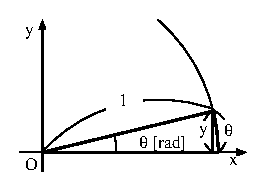
\includegraphics{math-images/small-sin.eps}}
%\begin{overpic}[width=5cm,grid,tics=10]{math-images/small-sin-nolabel.eps}
\begin{overpic}[width=5cm]{math-images/small-sin-nolabel.eps}
\put(5,3){$O$}
\put(92,3){$x$}
\put(4,60){$y$}
\put(45,28){$1$}
\put(85,2){$1$}
\put(77,18){$y$}
\put(52,13){$\theta$[rad]}
\put(89,17){$\theta$}
\end{overpic} 
\caption{$\theta\ll 1$のとき,$\sin\theta\simeq\theta$となる}
\label{fig:small-sin}
\end{center}
\end{figure}

\subsubsection{地球から月までの距離}

\nquestion
古代ギリシャ時代に\nmindex{ヒッパルコス}
(\nmindex{Hipparchos}, BC190-BC125頃)
\footnote{ヒッパルコスは天体観測のために正弦表も作成した
                                %Wikipedia 三角関数
}
は\textbf{地球から月までの距離}を以下のような方法で見積もった。
\begin{enumerate}
\item 同じ時刻に月が水平方向に見える地点と,真上に見える地点を探す
  \footnote{正確に時を刻む時計のなかったこの時代には,どうやって異なる
  地点で時の同時性を判断するかは大きな問題であった。たとえばどのような
  方法がありえるか各自考えてみよ}。
  この2点間と地球の中心のなす角度$\theta$がわかれば,月までの距離$x$が
  地球の半径$R$の何倍かを求めることが出来る。
  月までの距離$x$を地球の半径$R$と角度$\theta$を使って表しなさい。
  ここで,月までの距離$x$とは,月と地球の中心間の距離とする。
\item ヒッパルコスはその2地点と地球の中心のなす角度が89度であると結論
  づけ,地球の半径に対して地球と月の間の距離が何倍であるかを計算
  した。この値(概算値)を求めよ。
\item 地球のおおよその大きさは,ヒッパルコス以前にすでに見積もられてい
  た。
  地球が真円でありその周を40,000kmとした場合に
  \textbf{地球と月の間の距離}が何kmか概算で求めなさい。
  現在は地球と月の間の距離は約38.4万kmであることがわかっている。
\end{enumerate}
このように三角関数は,建物や山などから天体にいたるまで様々な対象の高さ
や距離や位置を測るために発達した。



%%%%%%%%%%%%%%%%%%%%%%%%%%%%%%%%%%%%%%%%%%%%%%%%%%%%%%%%%%%%%%%%%%%%%%%%%%%%%


\subsection{冪関数と指数関数}
\subsubsection{冪乗}

ある数$a$を何度か繰り返しかけて出来る数を$a$の\bfindex[べきじょう]{冪乗}(巾乗)
(\nmindex{power})もしくは単に\bfindex[べき]{羃}と呼ぶ。
$a$と自然数$n$に対して,$a$を$n$回掛ける演算は$a^n$と書き,
$a$を\bfindex[てい]{底}(\nmindex{base}), 
$n$を\bfindex[しすう]{指数}(\nmindex{exponent})と呼ぶ\footnote{$0^0$は
  通常定義しない。}。

また,正の自然数$n$に対して負の羃乗は以下のように定義される。
\begin{align}
  a^{-n}=(a^{-1})^n=\frac{1}{a^n}\notag
\end{align}

\nquestion
以下を証明しなさい。
\begin{enumerate}
\item $(x^n)^m=x^{n\times m}$
 \item $x^nx^m=x^{n+m}$
\item $x^0=1$
\end{enumerate}

%%%%%%
\subsubsection{冪関数}
$y=ax^k$ ($a, k$は定数)の形の関数を\textbf{冪関数}と呼ぶ。
冪関数は自然現象を表す法則にしばしば登場する。
たとえば,万有引力やクーロン力の大きさは冪関数で表される。

%%%%%%
\subsubsection{指数関数}
正の自然数$n$に対して
\begin{align}
  y=a^\frac{1}{n}, \quad(a>0)\notag
\end{align}
の値は\textbf{以下をみたす正の値}と定義される。
\begin{align}
  y^n=a,\quad (y>0)\notag
\end{align}
そこで,$a^\frac{n}{m}=\left(a^\frac{1}{m}\right)^n$と定めることにより,
羃乗の指数を任意の有理数とすることができる。
さらに指数を任意の実数$x$にまで拡張した関数
\begin{align}
f(x)=a^x,\quad (a>0)\notag
\end{align}
を\bfindex[しすうかんすう]{指数関数}(\nmindex{exponential function})
と呼ぶ。ここで,$a>0$ならば任意の$x$に対して$f(x)>0$である。
% $a$を\bfindex[てい]{底}(\nmindex{base}), 
% $x$を\bfindex[しすう]{指数}(\nmindex{exponent})と呼ぶ。

人口の増加の様子,放射性物質の崩壊による原子数の時間変化,
化学変化による物質量の変化など,さまざまな自然現象を指数関数で記述でき
ることが知られている。

%%%%%%
\exercise
以下を計算して簡単にしなさい
\answer{
(\ref{item:4^(3/2)}) 8~
(\ref{item:4^(-3/2)}) 1/8~
(\ref{item:(1/4)^(3/2)}) 1/8~
(\ref{item:(1/4)^(-3/2)}) 8~
(\ref{item:27^(2/3)^(1/2)}) 3~
(\ref{item:4^(e-sqrt2)/2^(-e+sqrt2)}) $2^e$~
% (\ref{item:(xy/x^4y^-1)^1/2}) $y/x$
}。
\begin{enumerate}
\item\label{item:4^(3/2)} $\displaystyle 4^\frac{3}{2}$
\item\label{item:4^(-3/2)} $\displaystyle 4^{-\frac{3}{2}}$
\item\label{item:(1/4)^(3/2)} $\displaystyle\left(\frac{1}{4}\right)^{\frac{3}{2}}$
\item\label{item:(1/4)^(-3/2)} $\displaystyle\left(\frac{1}{4}\right)^{-\frac{3}{2}}$
\item\label{item:27^(2/3)^(1/2)} $\displaystyle\left(27^{\frac{2}{3}}\right)^{\frac{1}{2}}$
\item\label{item:4^(e-sqrt2)/2^(-e+sqrt2)} $4^{e-\sqrt{2}}\times 2^{-e+2\sqrt{2}}$
% \item\label{item:(xy/x^4y^-1)^1/2} $\displaystyle\left(\frac{xy}{x^3y^{-1}}\right)^{\frac{1}{2}}$
\end{enumerate}

\subsubsection{平方根・冪根}

ある複素数$a$が与えられたとき, 2乗すると$a$になる数$x$, すなわち
\begin{align}
x^2=a\notag
\end{align}
を満たす数$x$を$a$の\bfindex[へいほうこん]{平方根}
(\nmindex{square root})とよぶ。

さらに, 複素数$a$と自然数$n$に対して, $n$乗すると$a$になる数$x$, すなわち
\begin{align}
x^n=a\notag
\end{align}
を満たす数$x$を$a$の\bfindex[えぬじょうこん]{$n$乗根}
(\nmindex{$n$-th root})とよぶ。
% 複素数の範囲内で$n$乗根は$n$個存在する。
また, 平方根や$n$乗根の総称を\bfindex[べきこん]{冪根}(べきこん)という。

%%%%%%
\subsubsection{根号}

ある\textbf{正の実数}$a$に対して,その\textbf{平方根のうち正の方}, す
なわち$\displaystyle a^{\frac{1}{2}}$を\bfindex[こんごう]{根
  号}$\sqrt{~}$を用いて
\begin{align}
  \sqrt{a}\quad(=a^{\frac{1}{2}})\notag
\end{align}
と書く。さらに\textbf{負の実数$a$に対しては}
\begin{align}
  \sqrt{a}=\sqrt{-|a|}=\sqrt{|a|}\;i\notag
\end{align}
と定義する。

また,$\sqrt[n]{a}$ ($n>2$)を以下のように定義する。
\begin{enumerate}
\item \textbf{正の実数}$a(>0)$に対して
\begin{align}
  \sqrt[n]{a}=a^\frac{1}{n}\notag
\end{align}
\item \textbf{負の実数}$a(<0)$に対して
\begin{align}
  \sqrt[n]{a}=
  \begin{cases}
    -\sqrt[n]{|a|} & n: 奇数\\
    未定義 & n: 偶数(実数の範囲にn乗根無し)
  \end{cases}\notag
\end{align}
\end{enumerate}

上記のように根号の定義式は複雑である。
基本的には,冪根のうち実数値を,実数値が複数あるときは正の値を採用する。
冪根が複素数のみのときには,平方根であれば虚部が正となる値を,平方根
以外であれば値なしとする。

\nquestion
以下をできるだけ簡単な形にしなさい
\answer{
(\ref{sqrt(-2)(-2)})~$2$~
(\ref{sqrt(-2)sqrt(-2)})~$-2$~
(\ref{item:sqrtx^2}) $|x|$
% (\ref{sqrt{-125}})~$\sqrt{5}$~
}。
\begin{enumerate}
\item\label{sqrt(-2)(-2)} $\displaystyle\sqrt{(-2)(-2)}$
\item\label{sqrt(-2)sqrt(-2)} $\displaystyle\sqrt{-2}\sqrt{-2}$
\item\label{item:sqrtx^2} $\displaystyle \sqrt{x^2}$
% \item\label{sqrt{-125}} $\displaystyle\sqrt[3]{-125}$
\end{enumerate}

\exercise
以下の値を求めなさい
\answer{
(\ref{item:sqrt4}) $\pm 2$~
(\ref{item:sqrt{4}}) $2$~
(\ref{item:4^1/2}) $2$~
(\ref{item:3rt-9}) $-2$~, $1\pm\sqrt{3}i$
(\ref{item:sqrt3{-8}}) $-2$~
(\ref{item:(-8)^1/3}) 未定義~
(\ref{item:4rt16}) $\pm 2$, $\pm 2i$~
(\ref{item:sqrt4{16}}) $2$~
(\ref{item:16^1/4}) $2$~
}。
\begin{enumerate}
\item\label{item:sqrt4} 4の平方根
\item\label{item:sqrt{4}} $\displaystyle\sqrt{4}$
\item\label{item:4^1/2} $\displaystyle 4^{\frac{1}{2}}$
\item\label{item:3rt-9} $-8$の$3$乗根
\item\label{item:sqrt3{-8}} $\displaystyle\sqrt[3]{-8}$
\item\label{item:(-8)^1/3} $\displaystyle (-8)^{\frac{1}{3}}$
\item\label{item:4rt16} 16の$4$乗根
\item\label{item:sqrt4{16}} $\displaystyle\sqrt[4]{16}$
\item\label{item:16^1/4} $\displaystyle 16^{\frac{1}{4}}$
\end{enumerate}

\subsubsection{ネイピア数}

% ある細菌が細胞分裂をして増殖をするとき,その細菌の数
% $n(t)$の時間変化をどのように表したら良いかを考えてみよう。

% 時刻$t$におけるこの細菌の数を$n(t)$とおく。
% 細菌が時間$T$たったときに1度細胞分裂をして, そのときに増加数がもとの数
% の$k$倍であったとすると, 
% \begin{align}
%   h(T)=(1+r)^nh_0
% \end{align}
% となる。
% 時間$T/2$毎に細胞分裂をするが, その度に増える割合は$\frac{r}{2}$

利子が$x$の一年複利で貯金をした場合,一年後に手に入れることが出来る金額が元の何倍か(貯金の増加率)を計算すると以下になる。
\begin{align*}
  (1+x)^1
\end{align*}
半年複利で利子$x/2$(半年当たり)で貯金した場合, 一年間での貯金の増加率は
\begin{align*}
  \displaystyle \left(1+\frac{x}{2}\right)^2
\end{align*}
である。
このように複利計算の期間をどんどん短くしていくと表\ref{tab:money}のようになる。
{\small
\begin{table}[t]
  \centering
  \caption{複利計算。利率は一回の複利計算あたりの値。}
  \label{tab:money}
  \begin{tabular}[h]{|c|c|cl|}\hline
         & 利率                        & 1年後          & $r=1.0$のとき\\\hline
1年複利  & $r$                         & $a_0(1+r)^1$    & ($=2a_0)$ \\
半年複利 & $\displaystyle\frac{r}{2}$  & $\displaystyle a_0\left(1+\frac{r}{2}\right)^2$&(=$2.25a_0$)\\
4ヶ月複利& $\displaystyle\frac{r}{3}$  & $\displaystyle a_0\left(1+\frac{r}{3}\right)^3$&(=$2.37a_0$)\\
$\vdots$ & $\displaystyle\vdots$       & $\vdots$ & \\
$1/n$年複利 & $\displaystyle\frac{r}{n}$   & $\displaystyle a_0\left(1+\frac{r}{n}\right)^n$&\\
$\vdots$ & $\displaystyle\vdots$       & $\vdots$  &\\\hline
  \end{tabular}
\end{table}
}
,さらに複利計算の期間をどんどん短くした極限($n\to\infty$)をとった場合の一年間の増加率は
\begin{align}
	\label{eq:Napier-exp}
  \lim_{n\to\infty} \left( 1 + \frac{x}{n} \right)^n
  \end{align}
となる。上式で利率を$x=1$ ($100\%$)とした場合の増加率を
\bfindex[ねいぴあすう]{ネイピア数}
\footnote{対数の発明者ジョン・ネイピアにちなんだ名称。
ネイピアが作成した対数表の底は$e$に非常に近い定義に基づく値であった。
上述のような複利計算に基づく$e$の定義は数学者
%\href{https://ja.wikipedia.org/wiki/%E3%83%A4%E3%82%B3%E3%83%96%E3%83%BB%E3%83%99%E3%83%AB%E3%83%8C%E3%83%BC%E3%82%A4}
{ヤコブ・ベルヌーイ}(Jakob Bernoulli, 1654-1705, スイス)による。ベルヌーイはライプニッツから微積分を学ぶ。
ネイピア数を記号$e$で初めて表したのはレオンハルト・オイラー(Lenhard Euler, 1704-1783)。
}
とよび,$e$で表す。その値は
\begin{align}
e=\lim_{n\to\infty}\left(1+\frac{1}{n}\right)^{n}=2.71828\cdots\notag  
\end{align}
と続く数であることが知られている。

$e$を用いると式(\ref{eq:Napier-exp})は
\begin{align}
	\label{eq:natural-exponential}
	e^x = \lim_{n\to\infty} \left( 1 + \frac{x}{n} \right)^n
\end{align}
と表すことができる。これがオイラーによる\bfindex[しぜんしすうかんすう]{自然指数関数}\footnote{底を$e$とする指数関数}の定義式である。さらに,この定義に基づき,底を$a$とする指数関数も以下のように計算できる。
\begin{align}
	\label{eq:euler-exponential}
	a^x=e^{x\cdot \ln a}
\end{align}

\nquestion 以下の問いに答えなさい。
\begin{enumerate}
\item 式(\ref{eq:Napier-exp})から式(\ref{eq:natural-exponential})を導きなさい。
\item 式(\ref{eq:euler-exponential})が成り立つことを証明しなさい。
\end{enumerate}
\comment
常に一定の割合で変化をするもの(利子,個体の大きさや数,崩壊する放射性
同位体等々)を数学的に扱うと,この$e$
\footnote{$e$の定義方法は他にもいくつかある。例えば
「微分方程式$y'(x)=y(x)$, $y(0)=1$を満たす解を$y=\exp x$とおいたとき,
$e=\exp 1$と定義する」といったものがある。}がしばしば現れる。

\subsection{対数関数}

\subsubsection{対数表:かけ算と割算}
例えば,16×8を計算するとき,
\begin{align}
  16\times 8=2^4\times 2^3=2^{4+3}=2^7\notag
\end{align}
と計算すると,かけ算を足し算に変換することができる。
はじめの16と8がそれぞれ2の何乗か
(それぞれ$\log_216$と$\log_28$\index{log}と書く)と,
最後の$2^7$の値は付録\ref{app:ln}のような\textbf{対数表}があ
れば簡単にわかる。

同様に14×17を計算すると次のようになる。
\begin{align}
  14\times 17&\simeq 2^{3.80735}\times 2^{4.08746}\notag\\
  &=2^{3.80735+4.08746}\notag\\
  &=2^{7.89481}\notag\\
  &\simeq 238\notag
\end{align}

\nquestion
対数表を用いて以下の計算をしなさい
\answer{
(\ref{item:128x64/4096}) 2~
(\ref{item:13x32x8}) 3328~
(\ref{item:128x138/184}) 96~
}。
\begin{enumerate}
\item\label{item:128x64/4096} $128\times 64\div 4096$
\item\label{item:13x32x8} $13\times 32\times 8$
\item\label{item:128x138/184} $128\times 138\div 184$%=2^{7+7.10852-7.52356}=96
\end{enumerate}

\comment
「\textbf{$a$を何乗したら$x$になるか}」を$\log_ax$で表す。
そして, これを\bfindex[たいすうかんすう]{対数関数}もしくは単に
\bfindex[たいすう]{対数}とよぶ。

このかけ算を足し算に変換する不思議な\textbf{対数}の概念は発明家ジョン・
\nmindex{ネイピア}(John Napier\index{Napier, John}, 1550-1617, スコットランド)
\footnote{ネイピアは様々な発明をしたことが知られているが,特に対数と少
  数点の発明で有名。}
によって発見された。
$\log$という表記は,ネイピアが対数を自然現象とは異なる純粋に論理上の演
算と考えて\bfindex{logistic algorithm} (\bfindex{logarithm})と名付けた
ことに起因するが, 後でも触れるように$\log$は自然現象の解析を行うと多く
の場面で必要になる重要な関数の一つである。

ネイピアは20年かけて\textbf{対数表}の作成も行った。
対数表を用いた計算方法は,計算機が発達する20世紀後半まで用い
られ,科学と工学のみならず文明の進歩に大きく貢献した。
よって正確な対数表の作成は国家プロジェクトとなる重要な事業であった。

% \nquestion [平方根と対数表]
% 対数表を使うとある数$x$の平方根や$n$乗根も簡単に求めることができる。
% \begin{enumerate}
% \item ある数$x$の$n$乗根を対数表を使って求める方法を考えなさい。
% %必要であれば $\log_a b^c=c\log_a b$を使っても良い
% %(\ref{sec:log-formula}節で証明)。
% \item 4096の2乗根,3乗根,4乗根を付録の対数表を使って求めなさい。
% \end{enumerate}

\subsubsection{対数関数の定義と基礎\label{sec:log-formula}}
\bfindex[たいすうかんすう]{対数関数}のより正確な定義は以下の通りである。
\begin{quote}
「ある正の数(真数)$x$が,別の正の数(底)$a(\ne 1)$を何乗したものか」
を
\begin{quote}
  $\log_a x$
\end{quote}
という記号で表し,$f(x)=\log_a x$を\textbf{対数関数}とよぶ。
\end{quote}
$y=\log_a x$ならば定義より$x=a^y$が成立する。
ここで指数関数の定義より$a>0$であり,また,$a=1$ではこれを何乗しても
1にしかならないので,底$a$は以下を満たすことが条件となる。
\begin{quote}
  $a>0$, $a\ne 1$
\end{quote}
さらに,$x=a^y>0$なので,真数$x$について$x>0$を満たすことが
対数関数の条件であり,これを\bfindex[しんすうじょうけん]{真数条件}とよ
ぶ。

また,対数関数の定義よりただちに,
\begin{quote}
  $y=\log_a x$の逆関数は$y=a^x$
\end{quote}
である。

指数関数の数式処理に困った時には対数表現に変形するとしばしば突破口が開
ける。
逆に対数関数の扱いに困ったら指数関数にしてみると良い。

%%%
\nquestion
以下のグラフを書きなさい。$a$の値によりその概形がどう異なるかを考え,
その特徴を場合分けをして示すこと。
\begin{enumerate}
\item $y=a^x$ ($a>0$)
\item $y=\log_ax$ ($a>0,a\ne 1$)
\end{enumerate}

\comment
底が$e$である対数$\log_e$は自然現象の解析で多く使われること
から\bfindex[しぜんたいすう]{自然対数} (\nmindex{natural logarithm})と
よび,しばしば$\ln$\index{$\ln$}と書く。
一方,底が$10$である対数$\log_{10}$は
\bfindex[じょうようたいすう]{常用対数}とよぶ。
単に$\log$と書く場合には,工学分野では常用対数($\log_{10}$)を指すこ
とが多いが,自然科学分野では自然対数($\log_e$)を指す。
\textbf{本テキストで以降単に$\log$と書いたときには自然対数を指す。}


%%%%%%%%%%%%
\subsubsection{対数関数の基本公式}

\nquestion
対数関数$\log$の定義より次式を証明せよ。以下で$a,b,c,x,y>0$である。
また,底の値は1ではないとする。
\begin{enumerate}
\item $\log_a 1=0$
\item $\log_a a=1$
\item $\log_a b^c=c\log_a b$
\item $\log_a xy=\log_a x+ \log_a y$
\item $\displaystyle\log_a c=\log_a b\cdot\log_b c$\quad
($\displaystyle\log_b c=\frac{\log_a c}{\log_a b}$)
\end{enumerate}

\exercise
% \begin{enumerate}
% \item 
以下を出来るだけ簡単な表現に直しなさい
\answer{
% (\ref{item:log_8}) 3~
(\ref{item:log_xy}) 1~
(\ref{item:log_log}) 1~
(\ref{item:log_23log_34}) 2~
(\ref{item:log_23}) 3~
(\ref{item:e^ln2}) 2~
(\ref{item:2^log}) 9~
% (\ref{item:3^log}) 2
}。
\begin{enumerate}
% \item \label{item:log_8}$\log_2 8$
\item \label{item:log_xy} $\log_315-\log_35$
\item \label{item:log_log} $\log_2(\sqrt{3}+1)+\log_2(\sqrt{3}-1)$
\item \label{item:log_23log_34} $\log_23\cdot\log_34$
\item \label{item:log_23}$2^{\log_23}$
%\quad(ヒント:$y=2^{\log_23}$とおいて$\log_2y$の値がどうなるか考える)
\item \label{item:e^ln2}$e^{\ln 2}$
\item \label{item:2^log}$2^{\log_{\sqrt{2}}3}$
% \item \label{item:3^log}$3^{\log_94}$
\end{enumerate}

%%%%%%%%%%%%%%%%%
% \begin{extra}
% \exercise
% 以下の数の大小関係を述べなさい\answer{
% $\log_\frac{1}{2}3
% <-1
% <\log_3\frac{1}{2}
% <0
% <\log_\frac{1}{3}\frac{1}{2}
% <1
% <\log_43
% <2
% <\log_326
% <3
% <\log_29$
% }。
% \begin{align}
%    -2, \;
%    &-1, \;
%    0, \;
%    1, \;
%    2, \;
%    3, \;
%    \log_29,\;
%    \log_326,\notag\\
%    &\log_43,\;
%    \log_\frac{1}{2}3,\;
%    \log_3\frac{1}{2},\;
%    \log_\frac{1}{3}\frac{1}{2}\notag
% \end{align}
% \end{extra}
%%%%%%%%%%%%%%

\subsubsection{対数方程式}
対数方程式を解くときには,
\begin{quote}
  $\log_a〇=△$
\end{quote}
対数関数の定義に基づいて指数関数を用いた形
($a^△=○$)に直すか,
\begin{quote}
  $\log_a〇=\log_a△$
\end{quote}
の形に変形したあと対数表現を用いない形($〇=△$)に
する。
一般には以下の手順で解く。
\begin{enumerate}
\item \textbf{真数条件}($\log_ax$において$x>0$)を確認する。
\item 底をそろえる。
\item 式を整理して,\textbf{対数を用いない表現}にして解を求める。
\item 解が真数条件を満たしているかを確認する。
\end{enumerate}
\exercise
以下の対数方程式を解きなさい
\answer{(1) $x=12$~ (2) $x=0$~(3) $x=2$  (真数条件に注意)~
  (4) $x=0$~ (5) $x=4,8$}。
\begin{enumerate}
\item $\log_2(x-4)=3$
\item $2=\ln (x+e^2)$
\item $\log_2x+3\log_8(x-1)=1$
%\item $\log_{\sqrt{2}}(x-2)-\log_2(3x-6)=1$ %(ans.x=8)
\item $\log_{\sqrt{3}}(x+3)-\log_9(3x+9)=1$
\item $\log_4x^2+6\log_x2=5$
\end{enumerate}

\subsubsection{対数不等式}
\nquestion
以下の各問の2つの対数はどちらが大きいか。
それぞれの値を計算して答えよ。
\begin{enumerate}
\item $\log_22$と$\log_24$
\item $\log_\frac{1}{2}2$と$\log_\frac{1}{2}4$
\end{enumerate}
\nquestion
以下がなりたつとき$p,q$の大小関係を述べよ
\answer{$0<a<1$のとき$p<q$, $1<a$のとき$p>q$ (グラフを描いて考えるとよい)}。
\begin{quote}
$\log_ap>\log_aq$, ($a>0$, $a\ne1$)
\end{quote}

\exercise
以下の対数不等式を解きなさい。
対数方程式で述べた計算手順を参照の上,真数条件に気を付けること
\answer{(1) $x>4$~(2) $0<x<4$~ (3) $x>\frac{1}{3}$~ (4)
  $0<x<3$~ (5) $1<x<2$ (真数条件に注意)}
。
\begin{enumerate}
\item $\log_2x>\log_24$
\item $\log_\frac{1}{2}x>\log_\frac{1}{2}4$
\item $\log_2x>\log_\frac{1}{4}9$
\item $\log_\frac{1}{2}x>\log_\frac{1}{4}9$
%\item $\log_\frac{1}{2}(x-1)>\log_\frac{1}{4}(7-x)$%ans. $1<x<3$ (真数条件に注意)}。
\item $\log_\frac{1}{3}(x-1)>\log_\frac{1}{9}(3-x)$
\end{enumerate}

\subsection{対数関数と指数関数の応用問題}

\subsubsection{対数グラフ}
点$(x,y)$をグラフ上に表したいとき, $x$軸の目盛を$\log x$(対数目盛)にとっ
たグラフを\bfindex[たいすうぐらふ]{対数グラフ}という。
特に, 横軸もしくは縦軸の片方のみを対数目盛にしたものを\bfindex[かたたいすうぐらふ]{片対数グラフ}, 
両方の軸を対数目盛にしたものを\bfindex[りょうたいすうぐらふ]{両対数グラフ}とよぶ。

例えば,$y=x^2$を両対数グラフにプロットするには,以下のように考えると良い。
$y=x^2$の両辺の対数をとると,次式が得られる。
\begin{align*}
\log y=2\log x
\end{align*}
ここで,$X=\log x$, $y=\log y$とおくと,上式は次式になる。
\begin{align*}
Y=2X
\end{align*}
ちょうど,この$X$, $Y$が両対数グラフの各軸を表すので,$y=x^2$は両対数グラフ上
では図\ref{fig:loglog-x2}のように傾き2の直線になる。

このように,なんらかの変数に対する指数関数は,通常のグラフでは曲線になるが,
両対数グラフでは指数を傾きとする直線になる。
そのため,様々な物理実験データを両対数グラフにプロットすることで,そのデータ点がなんらかの
指数関数により得られたのか,その場合には指数の値はいくらかを容易に知ることができる。

\begin{figure}[tb]
\centering
     \begin{overpic}[width=6cm]{x2_on_logx-logy.eps}
%      \begin{overpic}[grid,tics=10,width=6cm]{x2_on_logx-logy.eps}
        {
          \put(60,95){$y=x^2$}
          \put(52,-5){$x$}
          \put(-6,52){$y$}
          \put(3,0){$10^{-2}$}
          \put(20,0){$10^{-1}$}
          \put(38,0){$10^0$}
          \put(56,0){$10^1$}
          \put(74,0){$10^2$}
          \put(90,0){$10^3$}
          \put(-6,5){$10^{-2}$}
          \put(-6,22){$10^{-1}$}
          \put(-4,39){$10^0$}
          \put(-4,57){$10^1$}
          \put(-4,74){$10^2$}
          \put(-4,91){$10^3$}
        }
      \end{overpic}
    \caption{$y=x^2$の両対数グラフ\label{fig:loglog-x2}}
\end{figure}

%%%%%
\nquestion
以下の関数を両対数グラフにプロットしなさい。
\begin{enumerate}
\item $y=x^3$
\item $\displaystyle y=\frac{1}{x^2}$
\end{enumerate}

%%%%%
\nquestion
以下のグラフは,地震のマグニチュード$M$および地震が放出するエネルギー
$E$と,その規模の地震が起きる1年あたりの頻度$n$を示したものである。
\begin{quote}
  \begin{center}
    \resizebox{7cm}{!}{\includegraphics{math-images/Richter.eps}}\\
  \end{center}
    図 地震のマグニチュード(\textbf{上部}横軸),および
    地震が放出するエネルギー(\textbf{下部}横軸)と, 
    その規模の地震が起きる1年あたりの頻度(縦軸)を示す。
\end{quote}
\begin{enumerate}
\item マグニチュード$M$と地震の頻度$n$の関係式を書きなさい
  \answer{$n=a10^{-bM}$, ($a,b$は定数)}。
\item 地震のエネルギー$E$と地震の頻度$n$の関係式を書きなさい
  \answer{$n=aE^{-b}$, ($a,b$は定数)}。
\end{enumerate}


\subsubsection{対数と自然現象}
%%%%%%
\nquestion
地震の発するエネルギーの大きさ$E$と地震の
大きさを表すマグニチュード$M$には次式のような関係がある。
\begin{align}
  \log_{10}E=4.8+1.5M\notag
\end{align}
1995年の兵庫県南部地震(阪神・淡路大震災)のマグニチュードは7.0,
2011年の東北地方太平洋沖地震(東日本大震災)のマグニチュードは9.0であっ
た。後者の地震のエネルギーは前者の何倍か。
% \answer{\\1000倍}

%%%%%%
\nquestion
放射性同位体\footnote{構造が不安定で,時間と共に放射性崩壊していく原子の
  こと。}のある時点での原子数を$N$とすると,崩壊による原子数の減少の様子
は次式で表される。
\begin{align}
  \frac{dN}{dt}=-\lambda N\notag
\end{align}
ここで$\lambda$は定数である。この微分方程式を解くと次式が得られる。
\begin{align}
  \label{eq:halftime}
  N(t)=N_0e^{-\lambda t}
\end{align}
ここで$N_0$は時刻$t=0$での原子数である。

\begin{enumerate}
%\item 
% $N_0$と$\lambda$が既知の物質について,原子数$N(t)$より$t$を推定する式を導きなさい。
\item 
 原子数が半分になる時間(半減期)を$\tau$で表す。
 $\tau$が満たすべき方程式を$N(t)$を用いて表しなさい。
\item 
  $\tau=\displaystyle\frac{\ln 2}{\lambda}$となることを示しなさい。
\item 
 式(\ref{eq:halftime})を半減期$\tau$を用いて次式のように表すこと
  ができることを証明しなさい。
  \begin{align}
    \frac{N(t)}{N_0}=\left(\frac{1}{2}\right)^{\frac{t}{\tau}}\notag
  \end{align}
\end{enumerate}


%%%%%%%%%%%%%%%%%%
\subsubsection{対数と桁数}
%%%%%%
\nquestion 
$3^{20}$は10進数で何桁の数かを知りたい。以下の問いに答えなさい。
\begin{enumerate}
\item ある整数$a$が10進数で$b$桁の数であるとする。$x$が満たすべき条件式
  を書きなさい。\\
ヒント)このように一般化した表現を問われたときは,2桁の数がみたす条件
式は何かを具体的な数値を並べて考えるなど,考えやすい具体的な例で考えて
から,一般化して答えを導くのが常套手段
  \answer{$10^{b-1}\le a<10^{b}$}。
\item $3^{20}$は10進数で何桁の数か答えなさい
\answer{
  $3^{20}$は10進数で10桁の数。
}。
必要なら$\log_{10}3=0.4771$を使いなさい。
\end{enumerate}

%%%%%%%%%%%%%%%%%%
% \begin{extra}
% また,
% \begin{align}
% m^k\le n < m^{k+1}\notag
% \end{align}
% を満たすならば,$n$は$m$進数で$k+1$桁の数である。
% \end{extra}

% \begin{extra}
% \question
% 10および$3^{20}$が以下の各進数表示で何桁の数になるかを説明しなさい。
% 必要なら付録の対数表を参照しなさい
% \answer{
% 10は10進数で2桁,2進数で4桁,16進数で1桁。
% $3^{20}$は10進数で10桁,2進数で32桁,16進数で8桁。
% }。
% \begin{center}
% (1) 10進数\quad (2) 2進数\quad (3) 16進数
% \end{center}
% \end{extra}
%%%%%%%%%%%%%%%%%%%
\newpage

%%%%%%%%%%

\section{いろいろな座標表現}

$n$次元空間内のある点の位置は,しばしば直交する$n$個の座標系を用いて表さ
れる。このような座標系を
\bfindex[ちょっこうざひょう]{直交座標系}
(\nmindex{rectangular coordinate system})
もしくは\bfindex[デカルトざひょうけい]{デカルト座標系}
(\nmindex{Cartesian coordinate system})
\footnote{
  直交座標の発案者である
  \label{index:Descartes}
  デカルト(
  Ren\'{e} Descartes\index{Descartes, Ren\'{e}}, 
  1596-1650, 仏)  の名をとった呼び方。
  デカルトは哲学者,数学者であり,
  動物機械論,心身二元論を唱えた。また科学の手法として疑いようのない事実
  「我思うゆえに我あり」から全てを見直すことを提唱した。} 
と呼ぶ。

直交座標を用いるかわりに
ある基準点からの距離$r$ 
(\bfindex[どうけい]{動径}, \nmindex{radius})と方角
(\bfindex[へんかく]{偏角}, \nmindex{argument})
$\theta_1, \theta_2,\ldots,\theta_{n-1}$
を用いて位置を記述することもできる。
このような座標系を\bfindex[きょくざひょうけい]{極座標系}
(\nmindex{polar coordinate system})と呼ぶ。

\subsection{2次元極座標(円座標)}

\begin{figure}[h]
  \centering
%  \begin{overpic}[width=4cm,grid,tics=10]{math-images/polar.eps}
  \begin{overpic}[width=4cm]{math-images/polar.eps}
    \put(40,40){$O$}
    \put(67,54){$\theta$}
    \put(92,42){$x$}
    \put(42,95){$y$}
    \put(57,65){$r$}
    \put(78,82){$P$}
  \end{overpic}
  \caption{二次元極座標系}
  \label{fig:polar}
\end{figure}
二次元空間内の点Pの位置は,
原点$O$からの距離$r$
(\bfindex[どうけい]{動径})
と向き$\theta$(\bfindex[へんかく]{偏角})で記述することができる。
偏角$\theta$は,原点から始まる半直線を基準線とし,この半直線と線分OP
のなす角(反時計回りに測る)で表す。
ただし,原則として$0\le\theta<2\pi$とする。($-\pi<\theta\le\pi$を使う
場合もある)。
このように二次元空間内の座標を$(r,\theta)$の組で表す座標系を
\bfindex[にじげんきょくざひょう]{二次元極座標}, 
もしくは\bfindex[えんざひょう]{円座標}
(\nmindex{circular polar coordinates}),
\bfindex[きょくけいしき]{極形式}などとよぶ。
極座標の角度$\theta$を決定する基準線は,一般に直交座標系の$x$軸とする。

\nquestion
極座標$(r,\theta)$から直交座標$(x,y)$に変換する式を導きなさい
\answer{$(x,y)=(r\cos\theta,r\sin\theta)$}。
% \item 直交座標$(x,y)$から極座標$(r,\theta)$に変換する式を導きなさい。
% \answer{$(r,\theta)=(\sqrt{x^2+y^2},\cos^{-1}\frac{x}{\sqrt{x^2+y^2}})$. 
% ただし,$y\ge 0$のとき$0\le\theta<\pi$, $y<0$のとき$\pi\le\theta<2\pi$
% である。
% }。

\nquestion 以下の直交座標で表した各点を図示し, また
極座標で表しなさい
\answer{
(1) $(1,0)$~
(2) $(1,\frac{3}{2}\pi)$
(3) $(\sqrt{2},\frac{5}{4}\pi)$~
(4) $(2,\frac{7}{4}\pi)$~
(5) $(2,\frac{2}{3}\pi)$~
}。
\begin{enumerate}
\item $(1,0)$
\item $(0,-1)$
\item $(-1,-1)$
\item $(\sqrt{2},-\sqrt{2})$
\item $(-1,\sqrt{3})$
\end{enumerate}

\nquestion 以下の極座標で表した各点を図示し, また
直交座標で表しなさい
\answer{
(1) $(1,\sqrt{3})$
(2) $(2\sqrt{2},-2\sqrt{2})$~
(3) $(-1,0)$~
(4) $(-\sqrt{3},-1)$
(5) $(0,0)$
}。
\begin{enumerate}
\item $\displaystyle(2,\frac{\pi}{3})$
\item $\displaystyle(4,-\frac{\pi}{4})$
\item $\displaystyle(1,\pi)$
\item $\displaystyle(2,\frac{7}{6}\pi)$
\item $(0,3)$
\end{enumerate}

\nquestion 以下は2次元空間での直交座標と極座標の対応表である。
空欄を埋めなさい。解が複数の場合もあることに注意せよ
\answer{
(1) 0~
(2) 0~
(3) $\pm\sqrt{3}$
(4) $\displaystyle\frac{\pi}{6}$~($x=\sqrt{3}$のとき), 
    $\displaystyle\frac{5}{6}\pi$~($x=-\sqrt{3}$のとき)
(5) $\pm 2$
(6) $\displaystyle 0$~($x=2$のとき), 
    $\displaystyle\pi$~($x=-2$のとき)
(7) 0~
(8) 1~
(9) $1$~
(10) $\sqrt{2}$
}。
\begin{center}
  \begin{tabular}[h]{|c|c|c|}\hline
    直交座標 & 極座標\\\hline
    $(1,\sqbox)$ & $(1,\sqbox)$ \rule{0pt}{5mm}\\
    $(\sqbox,1)$ & $(2,\sqbox)$ \rule{0pt}{5mm}\\
    $(\sqbox,0)$ & $(2,\sqbox)$ \rule{0pt}{5mm}\\
    $(\sqbox,1)$ & $\displaystyle(\sqbox,\frac{\pi}{2})$ \rule{0pt}{5mm}\\
    $(1,\sqbox)$ & $\displaystyle(\sqbox,\frac{\pi}{4})$ \rule{0pt}{5mm}\\\hline
  \end{tabular}
\end{center}

%\subsection{いろいろな3次元座標系}

\subsection{3次元極座標(球座標)}

\begin{figure}[h]
  \begin{center}
    \resizebox{4.5cm}{!}{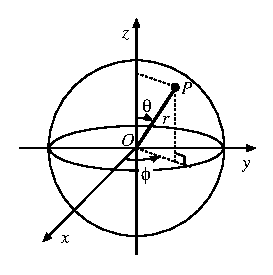
\includegraphics{math-images/polar-coord.eps}}
    \caption{3次元極座標系と直交座標系}
    \label{fig:polar-coord}
  \end{center}
\end{figure}
3次元空間内の点$P$の位置を,
図\ref{fig:polar-coord}のように原点$O$からの距離$r$(\textbf{動径})と, 
$OP$の$xy$平面への射影と$x$軸となす角$\phi$, $OP$と$z$軸のなす角
$\theta$の組$(r, \theta, \phi)$で表す座標表現を
\textbf{3次元極座標}もしくは\bfindex[きゅうざひょう]{球座標}
(\nmindex{spherical polar coordinates})という。
原則として$0\le\theta\le\pi$, $0\le\phi<2\pi$とする。

ただし,\textbf{3次元極座標系の角度の定義は教科書によってしばしば異なる}
  のでよく注意すること。
そして,本テキストのように, 
\textbf{3次元極座標系の$\theta$は2次元極座標系の$\theta$としばしば定義
  が異なる}ことにも注意せよ。

\question
% \begin{enumerate}
% \item
 極座標$(r, \theta, \phi)$から直交座標$(x, y, z)$への変換式を示し
  なさい
  \answer{$(x,y,z)=(r\sin\theta\cos\phi, r\sin\theta\sin\phi, 
  r\cos\theta)$}。
% \item 直交座標$(x, y, z)$から極座標$(r, \theta, \phi)$への変換式を示し
%   なさい
%   \answer{$(r,\theta,\phi)
%     =(\sqrt{x^2+y^2+z^2}, \cos^{-1}\frac{z}{\sqrt{x^2+y^2+z^2}},
%     \cos^{-1}\frac{x}{\sqrt{x^2+y^2}})$. 
%     ただし,$0\le\theta\le\pi$であり,$y\ge 0$のとき$0\le\phi\le\pi$,
%     $y<0$のとき$\pi<\phi<2\pi$である。
%     $x^2+y^2+z^2=0$ならば$\theta$と$\phi$は任意であるが,一般に
%     は$\theta=\phi=0$とする。
% }
% \end{enumerate}

% \subsubsection{円筒座標\prog}

% \begin{figure}[h]
%   \begin{center}
%     \resizebox{4.5cm}{!}{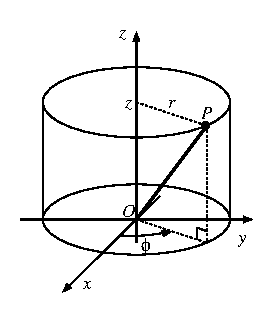
\includegraphics{math-images/cylinder-coord.eps}}
%     \caption{円筒座標系と直交座標系}
%     \label{fig:cylinder-coord}
%   \end{center}
% \end{figure}

% 図\ref{fig:cylinder-coord}のように,3次元空間内の点$P$の位置を$z$軸
% からの距離$r$, $OP$の$xy$平面への射影と$x$軸となす角$\phi$, $z$座標
% の組$(r, \phi, z)$で表す座標表現を\bfindex[えんちゅうざひょう]{円筒座
%   標}もしくは\bfindex[えんちゅうざひょう]{円柱座標}
% (\nmindex{cylindrical polar coordinates})という。
% \textbf{円筒座標系の動径$r$は極座標系の動径$r$と定義が異なることに注意せよ}。

% \question
%  円筒座標$(r, \phi, z)$から直交座標$(x, y, z)$への変換式を示し
%   なさい
%   \answer{$(x,y,z)=(r\cos\phi, r\sin\phi, z)$}。

% \question
% 直交座標$(x, y, z)$から円筒座標$(r, \phi, z)$への変換式を示し
%   なさい
%   \answer{$(r,\phi,z)=(\sqrt{x^2+y^2},\cos^{-1}\frac{x}{\sqrt{x^2+y^2}}, z)$. 
%     ただし,$y>0$のとき$0\le\phi\le\pi$であり, 
%     $y<0$のとき$\pi<\phi<2\pi$である。
%     $x^2+y^2=0$ならば$\phi$は任意であるが,一般に
%     は$\phi=0$とする。
% }。

\exercise
以下は3次元空間での直交座標と極座標の対応表である。
各点を図示し,また,空欄を埋めなさい
\answer{
(1) $\displaystyle(1,\frac{\pi}{2},0)$~~
(2) $\displaystyle(1,\frac{\pi}{2},\frac{\pi}{2})$~~
(3) $\displaystyle(\sqrt{2},\frac{3}{4}\pi,\frac{\pi}{2})$\\
(4) $\displaystyle(\frac{1}{\sqrt{2}},\frac{1}{\sqrt{2}},\sqrt{3})$~~
(5) $(-2,0,2)$~~
}。
\begin{center}
  \begin{tabular}{|c|c|}\hline
    直交座標 & 極座標 \prog\\\hline
    $(1,0,0)$ & $\qbox$ \rule{0pt}{5mm}\\
    $(0,1,0)$ & $\qbox$  \rule{0pt}{5mm}\\
    $(0,1,-1)$ & $\qbox$ \rule{0pt}{5mm}\\
    $\qbox$ & $\displaystyle(2,\frac{\pi}{6},\frac{\pi}{4})$ \rule{0pt}{5mm}\\
    $\qbox$ & $\displaystyle(2\sqrt{2},\frac{\pi}{4},\pi)$ \rule{0pt}{5mm}\\ \hline
  \end{tabular}
\end{center}

% 以下は3次元空間での直交座標,極座標,円筒座標の対応表である。
% 各点を図示し,また,空欄を埋めなさい
% \answer{
% (1) $\displaystyle(1,\frac{\pi}{2},0)$~~
% (2) $(1,0,0)$~~
% (3) $\displaystyle(1,\frac{\pi}{2},\frac{\pi}{2})$~~
% (4) $\displaystyle(1,\frac{\pi}{2},0)$~~\\
% (5) $\displaystyle(\sqrt{2},\frac{3}{4}\pi,\frac{\pi}{2})$~~
% (6) $\displaystyle(1,\frac{\pi}{2},-1)$~~
% (7) $\displaystyle(\frac{1}{\sqrt{2}},\frac{1}{\sqrt{2}},\sqrt{3})$\\
% (8) $\displaystyle(1,\frac{\pi}{4},\sqrt{3})$~~
% (9) $(-2,0,2)$~~
% (10) $\displaystyle(2\sqrt{2},\frac{\pi}{4},\pi)$~~
% % (11) $(\sqrt{3},\cos^{-1}\frac{1}{\sqrt{3}},\frac{\pi}{4})$~~
% % (12) $(\sqrt{2},\frac{\pi}{4},1)$~
% }。
% \begin{center}
%   \begin{tabular}{|c|c|c|}\hline
%     直交座標 & 極座標 & 円筒座標\prog\\\hline
%     $(1,0,0)$ & $\qbox$ & $\qbox$ \rule{0pt}{5mm}\\
%     $(0,1,0)$ & $\qbox$ & $\qbox$ \rule{0pt}{5mm}\\
%     $(0,1,-1)$ & $\qbox$ & $\qbox$ \rule{0pt}{5mm}\\
%     $\qbox$ & $\displaystyle(2,\frac{\pi}{6},\frac{\pi}{4})$& $\qbox$ \rule{0pt}{5mm}\\
%     $\qbox$ & $\qbox$ & $(2,\pi,2)$ \rule{0pt}{5mm}\\ \hline
% %     $(1,1,1)$ & $\qbox$ & $\qbox$ \\\hline
%   \end{tabular}
% \end{center}


\newpage
\section{複素数}

\subsection{虚数単位と複素数}
2乗すると$-1$になる数を\textbf{虚数単位(imaginary unit)}と定義し,$i$
で表す\footnote{回路学等の工学分野では,電流を$i$と表すことが多いので,
  虚数単位を$j$と書くこともある。}。すなわち,\textbf{虚数単位}$i$は次
  式を満たす\textbf{想像上の数}である\footnote{二乗すると$-1$になる数
    は二つ存在するが, いずれか一方を$i$とおけば, もう一方は$-i$となる。}。
\begin{align}
  i^2=-1\notag
\end{align}
虚数単位は平方根を用いると次式のように表される。
\begin{align}
  i=\sqrt{-1}\notag
\end{align}
また,実数(real number) $a,b$と虚数単位$i$により
\begin{align}
  z=a+bi\notag
\end{align}
と表される数を\bfindex[ふくそすう]{複素数}
(\bfindex{complex number})とよぶ。
\textbf{実数空間は複素数空間の部分集合}である。

複素数$z$の
\bfindex[じっすうぶぶん]{実数部分}(\nmindex{real part})は
$\Re (z)$\index{$\Re$}, 
\bfindex[きょすうぶぶん]{虚数部分}(\nmindex{imaginary part})は
$\Im (z)$\index{$\Im$}で表す。
たとえば,
\begin{align}
z=a+bi \notag
\end{align}
ならば
\begin{align}
  \begin{cases}
    \Re (z)=a\\
    \Im (z)=b
  \end{cases}\notag
\end{align}
である。
特に,$\Re (z)=0$, $\Im (z)\ne 0$のとき,$z$を\bfindex[じゅんきょすう]{純虚数}
(\nmindex{purely imaginary number})と呼ぶ。

\nquestion\label{eq:eq-complex}
以下の式の解を求めなさい。
\begin{enumerate}
\item $x^2+2x+2=0$
\item $x^3=1$
\item $x^4=1$
\end{enumerate}

\comment 上の設問にあった二次方程式の2根のように,虚数部分の符号の
みが異なる2つの複素数を「互いに\bfindex[ふくそきょうやく]{複素共役}で
ある」という。
また,複素数$z=a+bi$と複素共役な複素数を\textbf{共役複素数}
(きょうやくふくそすう, \nmindex{complex conjugate})と呼び,一般に$\bar{z}(=a-bi)$と表す。

\nquestion
2つの複素数$z_1,z_2$について以下が成り立つことを証明しなさい。
\begin{align}
  \overline{z_1z_2}=\bar{z}_1\bar{z}_2\notag
\end{align}

\exercise
% \begin{enumerate}
% \item
 以下の式を出来るだけ簡単な形($a+bi$の形)にしなさい
\answer{
(\ref{iitem:(2+i)^2}) $3+4i$~
% (\ref{iitem:(2+i)(2-i)}) $5$~
(\ref{iitem:(2+i)/i}) $1-2i$~
% (\ref{iitem:2i/(1+i)}) $1+i$~
(\ref{iitem:(1+i)/(1-i)}) $i$
}。
  \begin{enumerate}
  \item\label{iitem:(2+i)^2} $(2+i)^2$
%   \item\label{iitem:(2+i)(2-i)} $(2+i)(2-i)$
  \item\label{iitem:(2+i)/i} $\displaystyle\frac{2+i}{i}$
%   \item\label{iitem:2i/(1+i)} $\displaystyle\frac{2i}{1+i}$
  \item\label{iitem:(1+i)/(1-i)} $\displaystyle\frac{1+i}{1-i}$
  \end{enumerate}
% \end{enumerate}

\subsection{複素平面}

\begin{figure}[h]
  \centering
%  \begin{overpic}[width=4cm,grid,tics=10]{math-images/complex-polar.eps}
  \begin{overpic}[width=4cm]{math-images/complex-polar.eps}
    \put(12,10){$O$}
    \put(90,6){$Re$}
    \put(8,92){$Im$}
    \put(40,55){$|z|$}
    \put(75,84){$z=a+bi$}
    \put(68,11){$a$}
    \put(13,75){$b$}
  \end{overpic}
  \caption{複素平面}
  \label{fig:complex}
\end{figure}

ある複素数$z=a+bi$が与えられたとき,点$(a,b)$を二次元
の座標平面上の点に対応させることができる(図\ref{fig:complex})。
このような平面を\bfindex[ふくそへいめん]{複素平面}
(\nmindex{complex plane})とよぶ。

\subsection{複素数の大きさ・距離}
\textbf{複素数$z$の大きさ(絶対値)}
\index{ふくそすう@複素数!のおおきさ@---の大きさ}
(\nmindex{absolute value}, \nmindex{modulus})は
複素平面上で$z$を表した
\textbf{点と原点との間の距離}で定義され,
$|z|$で表す。
$z=a+bi$の大きさは次式で与えられる。
\begin{align}
  |z|=\sqrt{a^2+b^2}\notag
\end{align}

また, 複素平面上での2点
\begin{align}
P:&\; z_1=a_1+b_1i\notag\\
Q:&\; z_2=a_2+b_2i\notag
\end{align}
の間の\bfindex[きょり]{距離}(\nmindex{distance})$\overline{PQ}$
は実数空間の場合と同様に次式で与えられる。
\begin{align}
  \overline{PQ}=|z_1-z_2|=
  \sqrt{(a_1-a_2)^2+(b_1-b_2)^2}\quad\cdots(*)\notag
\end{align}

\nquestion
\begin{enumerate}
\item 次式が成り立つことを証明しなさい。
  \begin{align}
    |z|=\sqrt{z\bar{z}}\notag
  \end{align}
\item (*)式で示したように,複素平面上の2点$z_1$, $z_2$の間の距離
  $\overline{PQ}$は,$z_1-z_2$の大きさ$|z_1-z_2|$と等しいことを示しな
  さい。
\end{enumerate}

\exercise
\begin{enumerate}
\item 次の複素数について以下の問に答えなさい。
  \begin{align}
    z_1&=1\notag\\
    z_2&=1+i\notag
  \end{align}
  \begin{enumerate}
  \item $z_1$, $z_2$とその共役複素数を複素平面上に描きなさい。
    また,それらの大きさを求めなさい。
  \item 以下の2点間の距離を求めなさい
    \answer{
      $|z_1-z_2|=1,$~
      $|z_2-\overline{z_2}|=2$
%       $|z_2-\overline{z_3}|=3$
      $|2z_2-1|=\sqrt{5}$
    }。
    \begin{enumerate}
    \item $z_1$と$z_2$
    \item $z_2$と$\overline{z_2}$
%     \item $z_2$と$\overline{z_3}$
    \item $2z_2$と$1$
    \end{enumerate}
  \end{enumerate}
\item 以下の方程式の解を複素平面に図示しなさい。
  \begin{enumerate}
  \item $x^3=1$
  \item $x^4=1$
  \item $x^2+2x+1=0$
  \end{enumerate}
\item 方程式 $x^2+2x+1-\epsilon=0$の解が,$\epsilon$の値によって
  複素平面をどのように動くか説明しなさい。
\end{enumerate}

% \newpage
% \rule{0pt}{10pt}
\subsection{複素平面の極座標表現\label{sec:complex-polar}}
\begin{figure}[h]
  \centering
%  \begin{overpic}[width=4cm,grid,tics=10]{math-images/complex-polar.eps}
  \begin{overpic}[width=4cm]{math-images/complex-polar.eps}
    \put(12,10){$O$}
    \put(47,27){$\theta=\arg z$}
    \put(90,6){$Re$}
    \put(8,92){$Im$}
    \put(40,55){$|z|$}
    \put(75,84){$z=a+bi$}
    \put(68,11){$a$}
    \put(13,75){$b$}
  \end{overpic}
  \caption{複素平面と極座標表現}
  \label{fig:complex-polar}
\end{figure}
複素平面において,複素数と原点を結ぶ直線と,実数軸の正の向きとなす角を
複素数$z=a+bi$の\textbf{偏角}
\index{ふくそすう@複素数!のへんかく@---の偏角}
と呼び,$\arg z$と表す。
ただし角度は反時計回り方向を正の方向とする(図\ref{fig:complex-polar})。
% 複素数$z=a+bi$の偏角を$\theta$とおくと,
%   \begin{align}
%     \label{eq:complex}
%     z=|z|(\cos\theta+i\sin\theta)
%   \end{align}
% と書くことができる。
複素数$z$の座標は\textbf{極座標形式}によって$(|z|,\arg z)$と表すことが
できる。

例えば$z=1+i$に対して, 
\begin{align}
  |z|=\sqrt{2},\quad \arg z=\frac{\pi}{4}+2n\pi,\quad(n\mbox{: 整数})\notag
\end{align}
なので,$z=1+i$を極座標形式で表すと以下のようになる。
\begin{align}
\left(\sqrt{2},\;\frac{\pi}{4}+2n\pi\right),\quad(n\mbox{: 整数})\notag
\end{align}

% 上記の$z=1+i$の偏角は以下のように表すことができる。
% \begin{align}
% \arg z=\frac{\pi}{4}+2n\pi,\quad(n\mbox{:整数})\notag
% \end{align}


\nquestion
次の複素数について以下の問に答えなさい。
\begin{align}
  z_1&=1\notag\\
  z_2&=-1+i\notag
%   z_3&=-2-i\notag
\end{align}

\begin{enumerate}
\item $z_1$, $z_2$を極座標形式で表しなさい。
\item $z_1$, $z_2$に以下の数をかけた値を極座標形式で答えなさい。
  また,複素平面上に描きなさい.
  \begin{enumerate}
  \item $2$
  \item $i$
  \item $2i$
  \item $z_2$
  \end{enumerate}
\item 複素数$z$に上記の数をかけるのは,複素平面上で$z$を
どのように移動させることになるか,説明しなさい。
\end{enumerate}

% \begin{extra}
% \question
% $z_1=\sqrt{3}+i$, $\displaystyle z_2=\frac{1}{2}(1+\sqrt{3}i)$として以
% 下の問に答えなさい。
% \begin{enumerate}
% \item $z_1$, $z_2$を複素平面上にプロットしなさい。
% \item  $z_1$, $z_2$の大きさと偏角を求めて, 各複素数を
%   極座標形式で表しなさい\answer{
% $\displaystyle z_1: \left(2,\frac{\pi}{6}+2n\pi\right)$,\;
% $\displaystyle z_2: \left(1,\frac{\pi}{3}+2n\pi\right)$,\;
% ($n$は整数)
% }。
% \item 以下をそれぞれ複素平面上にプロットしなさい。
% また, 各座標を極座標形式で表しなさい
% \answer{
% $\displaystyle P: \left(2,-\frac{\pi}{6}+2n\pi\right)$~
% $\displaystyle Q: \left(\sqrt{3},2n\pi\right)$~
% $\displaystyle R: \left(1,\frac{\pi}{2}+2n\pi\right)$~\\
% $\displaystyle S: \left(2,\frac{\pi}{2}+2n\pi\right)$~
% $\displaystyle T: \left(8,\frac{\pi}{2}+2n\pi\right)$~
% $\displaystyle U: \left(1,\frac{\pi}{3}+2n\pi\right)$\\
% ($n$は整数)
% }。
%   \begin{enumerate}
%   \item $\displaystyle P: \bar{z}_1$
%   \item $\displaystyle Q: \frac{z_1 + \bar{z}_1}{2}$
%   \item $\displaystyle R: \frac{z_1 - \bar{z}_1}{2}$
%   \item $\displaystyle S: z_1z_2$
%   \item $\displaystyle T: z_1^3$
%   \item $\displaystyle U: z_1/\bar{z}_1$
%   \end{enumerate}
% \end{enumerate}
% \end{extra}

複素数の演算の幾何学的意味は「数学の基礎訓練II」
%\ref{sec:Euler-complex}節
でより詳細に取り上げる。

%%%%%%
\nquestion
ある複素数$z$と複素数$i$の間の距離は
複素数$z$の大きさと丁度等しい。
\begin{enumerate}
\item 題意をもっともよく表す方程式を書きなさい
  \answer{$|z-i|=|z|$}。
\item 題意を満たす複素数が複素平面上で描く図形と, $\Re\{z\}=2$の交点を表
  す複素数を求めなさい
  \answer{$z=2+\frac{i}{2}$}。
\end{enumerate}

%%%%%%
\nquestion
ある複素数$z$を複素平面上において,原点に関して反時計回りに$\pi/2$回転した値と, 
$z$の共役複素数が等しくなる。
\begin{enumerate}
\item 題意をもっともよく表す方程式を書きなさい。
\answer{$iz=\bar{z}$}
\item 題意をみたす$z$を求めなさい。ただし$|z|=2$であるとする。
\answer{$z=\pm\sqrt{2}(1-i)$}
\end{enumerate}


\newpage

\section{いろいろな関数とグラフ}

\subsection{偶関数と奇関数}
任意の$x$について
\begin{align}
  f(x)=f(-x)\notag
\end{align}
が成り立つ関数$f(x)$を\bfindex[ぐうかんすう]{偶関数}
(\nmindex{even function})とよび,
\begin{align}
  f(x)=-f(-x)\notag
\end{align}
が成り立つ関数$f(x)$を\bfindex[きかんすう]{奇関数}
(\nmindex{odd function})とよぶ。

\nquestion
偶関数,奇関数の幾何学的意味を説明しなさい。

\nquestion
以下の関数を (a)偶関数,(b)奇関数,(c)どちらでもない, 
に分類しなさい\answer{
\textbf{(a)} 1, 3, 5, 7, 9~
\textbf{(b)} 2, 8~
\textbf{(c)} 4, 6~
}。
以下で$\exp x$は$e^x$を意味する。

\begin{tabular}{rcrcrc}
(1) & $x^2$ & (2) & $\sin x$ & (3) & $\cos x$ \\
(4) & $\exp x$ & (5) & $\sin^2 x$ & (6) & $\ln x$  \\
(7) & $\exp(-x^2)$ & (8) & $\displaystyle\frac{e^x-e^{-x}}{2}$ & 
(9) & $\displaystyle\frac{\sin x}{x}$
\end{tabular}

\subsection{関数の概形\label{sec:graph}}

\subsubsection{概形の書き方の基本}
以下の関数の概形を描きなさい。
\begin{enumerate}
\item $\displaystyle y=\frac{1}{1+e^{-x}}$
% \item $\displaystyle y=\frac{e^x-e^{-x}}{2}$
\item $\displaystyle y=\frac{e^x-e^{-x}}{e^x+e^{-x}}$\label{eq:tanh}
\end{enumerate}
\comment
概形を書くときには以下をチェックすること。
\begin{itemize}
\item 偶関数もしくは奇関数か? いずれかであれば$x\ge 0$の図を描ければ
  $x<0$もすぐ描ける。
\item 単調増加もしくは単調減少?
  \begin{enumerate}
  \item 単調性が確認できなかったら,起伏の様子を調べること。
  \item 判断のために必ずしもわざわざ微分を求める必要はない。せずにすむ
  計算はしないほうが間違いが減る。
  \end{enumerate}
\item $x\to\pm\infty$での関数値は? (奇関数や偶関数なら$x\to\infty$のみ
  でOK)
\item $x=0$での関数値は?
\end{itemize}

\subsubsection{複雑な関数の概形}
以下の関数の概形を描きなさい。
複雑な関数のグラフは,各パーツに分解して考えるとよい。
\begin{enumerate}
\item $\displaystyle y=\frac{e^x+e^{-x}}{2}$
  \\($\displaystyle y=\frac{e^x}{2}$と
  $\displaystyle y=\frac{e^{-x}}{2}$のグラフを足す)
\item $y=e^{-x}\sin x$
  \\($y=\sin x$と$y=e^{-x}$のグラフをかける)
\end{enumerate}

\subsection{関数の平行移動と拡大}

\nquestion
$y=\sin x$を以下のように変換した式とグラフをそれぞれ書きなさい
\answer{
(\ref{item:MoveSin}) $y=\sin (x-\frac{\pi}{2})$~
(\ref{item:StretchSin}) $y=\sin\frac{x}{2}$~
(\ref{item:MoveSinY}) $y-1=\sin x$~
(\ref{item:StretchSinY}) $\frac{y}{2}=\sin x$~
(\ref{itme:StretchMove}) $y=\sin \frac{x-\frac{\pi}{2}}{2}$~
(\ref{item:MoveStretch}) $y=\sin (\frac{x}{2}-\frac{\pi}{2})=\sin \frac{x-\pi}{2}$
}。
\begin{enumerate}
\item\label{item:MoveSin} $x$軸方向に$\displaystyle\frac{\pi}{2}$平行移動する。
\item\label{item:StretchSin} $x$軸方向に2倍に拡大する。
\item\label{item:MoveSinY} $y$軸方向に$1$平行移動する。
\item\label{item:StretchSinY} $y$軸方向に2倍に拡大する。
\item\label{itme:StretchMove} $x$軸方向に2倍に拡大してから,$x$軸
  方向に$\displaystyle\frac{\pi}{2}$平行移動する。 
\item\label{item:MoveStretch} $x$軸方向に$\displaystyle\frac{\pi}{2}$
  平行移動してから,$x$軸方向に2倍に拡大する。
\end{enumerate}

\nquestion 以下の問に答えなさい
\answer{
(\ref{item:MoveX}) $y=f(x-a)$~
(\ref{item:StretchX}) $y=f(x/c)$~
(\ref{item:MoveY}) $y-b=f(x)$~
(\ref{item:StretchY}) $y/d=f(x)$
}。
\begin{enumerate}
\item\label{item:MoveX}
 関数$y=f(x)$を$x$軸の正の方向に$a$だけ平行移動した関数の方程式を書き
  なさい。
\item\label{item:StretchX}
  関数$y=f(x)$を$x$軸方向に$c$倍に拡大した関数の方程式を書き
  なさい。
\item\label{item:MoveY}
  関数$y=f(x)$を$y$軸の正の方向に$b$だけ平行移動した関数の方程式を書き
  なさい。
\item\label{item:StretchY}
 関数$y=f(x)$を$y$軸方向に$d$倍に拡大した関数の方程式を書き
  なさい。
\end{enumerate}

\nquestion
以下の関数を表す式と概形を書きなさい。
\begin{enumerate}
\item 関数$y=x^2-2x+1$を$x$軸方向に$-1$だけ平行移動した関数
\item $x^2+4y^2=1$で表される図形を$y$軸方向に$\frac{1}{2}$倍した図形
\end{enumerate}

\nquestion
以下の関数の概形を書きなさい。
\begin{enumerate}
  % \item $\displaystyle y=\sin(x-\frac{\pi}{2})$\\
  %   ($y=\sin x$をどのように移動したか考える)
  % \item $\displaystyle y=\cos(x+\frac{3}{2}\pi)$\\
  %   ($y=\cos x$をどのように移動したか考える)
  % \item $\displaystyle y=\sin 2x$
  % \item $\displaystyle 2y=\sin x$
\item
  $\displaystyle y=\frac{e^{x-1}-e^{-x+1}}{e^{x-1}+e^{-x+1}}+2$\\
  (\ref{sec:graph}節の式(\ref{eq:tanh})をどのように移動したグラ
  フか考える)
\item $\displaystyle y=\frac{1}{1+e^{-\frac{x-h}{T}}}$,
  \quad($h,T$:定数) \\
  $T(>0)$の大きさによりグラフの形がどのように変わるかも図示すること。
  % この関数のような概形はシグモイド関数と呼ばれている。
\end{enumerate}

\subsection{逆関数}
関数$y=f(x)$を変形して,出力$y$に対応する$x$を求めることができる形に書
き直したものを
\begin{align}
  x=f^{-1}(y)\notag
\end{align}
と書く。
さらに記号$x$, $y$を入れかえて作った関数
\begin{align}
  y=f^{-1}(x)\notag
\end{align}
を関数$f(x)$の\bfindex[ぎゃくかんすう]{逆関数}と呼ぶ。

\comment
$y=\sin x$, $y=\cos x$の逆関数はそれぞれ
$y=\sin^{-1} x$, $y=\cos^{-1}x$,もしくは$y=\arcsin x$, $y=\arccos x$と書く。

\nquestion
以下の値を求めなさい
\answer{
(\ref{item:arcsin-1}) $\pi/2$~
(\ref{item:arcsin1/2}) 
$\frac{\pi}{6}+2n\pi,\frac{5\pi}{6}+2n\pi$~($n$は整数)~
% (\ref{item:arccos0}) $\frac{\pi}{2}$
(\ref{item:arccos1/2}) $\pm\frac{\pi}{3}+2n\pi$~($n$は整数)
}。
\begin{enumerate}
\item\label{item:arcsin-1} $\sin^{-1}1$ (値域を
  $\displaystyle[-\frac{\pi}{2},\frac{\pi}{2}]$\quad
\footnote{ある値$x$が$[a,b]$の値であるとは,$a\le x\le b$を意味する}とする)
\item\label{item:arcsin1/2} $\displaystyle\sin^{-1}\frac{1}{2}$\quad (値域を$(-\infty,\infty)$
\footnote{ある値$x$が$(a,b)$の値であるとは,$a< x< b$を意味する}とする)
% \item\label{item:arccos0}$\cos^{-1}0$\quad (値域を$[0,\pi]$とする)
\item\label{item:arccos1/2} $\displaystyle\cos^{-1}\frac{1}{2}$\quad (値域を$(-\infty,\infty)$とする)
\end{enumerate}

\nquestion
以下の逆関数を図示しなさい。
\begin{enumerate}
\item $y=\sin x$\quad $\displaystyle(-\frac{\pi}{2}\le x \le\frac{\pi}{2})$
\item $y=\cos x$\quad $\displaystyle(0\le x \le \pi)$
\end{enumerate}

\nquestion
任意の$x$に対して$\cos^{-1}x=\sin^{-1}x+a$, ($a:$~定数)が成り立つ$a$の
値を求めなさい。ただし, $0\le a<2\pi$とする。

\nquestion
以下の逆関数を求めよ。また,もとのグラフとその逆関数を同じ座標軸上に描
きなさい
\answer{
(\ref{item:inv(xx-2x)}) $y=\sqrt{x+1}+1$
(\ref{item:inv(expx)}) $y=\ln x$
% (\ref{item:inv(ax)}) $y=\log_ax$
(\ref{item:inv(ln(x+1))}) $y=e^x-1$
(\ref{item:inv(2sin3x)}) $y=\frac{1}{3}\sin^{-1}\frac{x}{2}$
(\ref{item:inv(2f(3x))}) $y=\frac{1}{3}f^{-1}(\frac{x}{2})$
}。
% $y=x$に対して対称なことを示しなさい。
\begin{enumerate}
\item\label{item:inv(xx-2x)} $y=x^2-2x$\quad $(x \geq 1)$
\item\label{item:inv(expx)} $y=e^x$
% \item\label{item:inv(ax)} $y=a^x$\quad$(a>0)$
\item\label{item:inv(ln(x+1))} $y=\ln (x+1)$\quad$(x>-1)$
\item\label{item:inv(2sin3x)} $y=2\sin 3x$
\item\label{item:inv(2f(3x))} $y=2f(3x)$
\end{enumerate}

\subsection{いろいろな図形表現}
\subsubsection{パラメータ関数のグラフ}

\question
各式があらわすグラフを2次元$xy$平面に描きなさい。
\begin{enumerate}
\item 
$    \begin{cases}
      x=t\\
      y=-2t+2
    \end{cases}(t\mbox{は任意の実数})$
\item 
$    \begin{cases}
      x=\cos\theta\\
      y=\sin\theta -2
    \end{cases}(\theta\mbox{は任意の実数})$
\end{enumerate}

% \subsection{極座標で表したグラフ}
\subsubsection{2次元極座標による図形表現}
\question
2次元$(r,\theta)$極座標系で以下のように表される図形の概形を書きなさい。
  \begin{enumerate}
  \item $r=1$
  \item $r=\theta$\quad ($\theta\ge 0$)
  \item $\displaystyle r=\cos\theta\quad (-\frac{\pi}{2}\le\theta\le\frac{\pi}{2}$)
  \end{enumerate}

\subsubsection{3次元極座標による図形表現}
\question
3次元$(r,\theta,\phi)$極座標系で以下のように表される図形の概形を書き
なさい。
\begin{enumerate}
\item $r=1$
\item $\theta=\displaystyle\frac{\pi}{3}$
\item
  $\begin{cases}
    r=\phi\quad(r>0)\\
    \theta=\displaystyle\frac{\pi}{3}
  \end{cases}
  $
\end{enumerate}

% \subsubsubsection{3次元極座標(円筒座標)\prog}
% \question 円筒座標系で以下のように表される図形の概形を書きなさい。
% \begin{enumerate}
% \item $r=1$
% \item $\theta=\frac{\pi}{3}$
% \item $
%   \begin{cases}
%     r=1\\
%     \theta=z
%   \end{cases}
%   $
% \end{enumerate}

\subsubsection{複素平面におけるグラフ}
以下の複素数$z=x+iy$が表すグラフを複素平面上に描きなさい。
\begin{enumerate}
\item $\Re(z)=1$
\item $z=1$
\item $z=i$
\item $|z|=1$
\item $|2z-1|=1$
\item $|z-2i|=2$
\item $z=(1+i)t$\quad ($t$は任意の実数)
\end{enumerate}

%\subsection{図形の数式による表現}
%以下の\textbf{定性的表現}による図形の表面を,
%数式による表現(\textbf{定量的表現})にしなさい。
%座標空間のどこにどの向きに図形を配置するかは,記述が出来るだけ簡潔にな
%るように工夫して決めなさい。
%\begin{enumerate}
%\item 一辺の長さ1の立方体
%\item 底面の半径1,高さ1の円筒
%\item 底面の半径1,高さ1の円錐
%\item 底面が正方形(一辺の長さ1),高さ1のピラミッド型(四角錐)
%\end{enumerate}

  
%%%%%%%%%%%%%%%%%%%%%%%%%%%%%%%%5
%\newpage
\rule{0pt}{10cm}
\newpage

\appendix
\section{対数表\label{app:ln}}
%% \begin{table}[htbp]
{\footnotesize
%\small
\begin{tabular}[h]{|cc|cc|cc|cc|cc|c|cc|cc|cc|}\hline
n&$\log_2n$&n&$\log_2n$&n&$\log_2n$&n&$\log_2n$&n&$\log_2n$&
&n&$\log_2n$&n&$\log_2n$ \\ \hline
1&0&51&5.67243&100&6.64386&151&7.2384&201&7.65105& &3300&11.68825&4051&11.98406\\ 
2&1&52&5.70044&101&6.65821&152&7.24793&202&7.65821& &3301&11.68869&4052&11.98442\\ 
3&1.58496&53&5.72792&102&6.67243&153&7.25739&203&7.66534& &3302&11.68912&4053&11.98477\\ 
4&2&54&5.75489&103&6.6865&154&7.26679&204&7.67243& &3303&11.68956&4054&11.98513\\ 
5&2.32193&55&5.78136&104&6.70044&155&7.27612&205&7.67948& &3304&11.69&4055&11.98549\\ 
6&2.58496&56&5.80735&105&6.71425&156&7.2854&206&7.6865& &3305&11.69043&4056&11.98584\\ 
7&2.80735&57&5.83289&106&6.72792&157&7.29462&207&7.69349& &3306&11.69087&4057&11.9862\\ 
8&3&58&5.85798&107&6.74147&158&7.30378&208&7.70044& &3307&11.69131&4058&11.98655\\ 
9&3.16993&59&5.88264&108&6.75489&159&7.31288&209&7.70736& &3308&11.69174&4059&11.98691\\ 
10&3.32193&60&5.90689&109&6.76818&160&7.32193&210&7.71425& &3309&11.69218&4060&11.98726\\ 
11&3.45943&61&5.93074&110&6.78136&161&7.33092&211&7.7211& &3310&11.69262&4061&11.98762\\ 
12&3.58496&62&5.9542&111&6.79442&162&7.33985&212&7.72792& &3311&11.69305&4062&11.98797\\ 
13&3.70044&63&5.97728&112&6.80735&163&7.34873&213&7.73471& &3312&11.69349&4063&11.98833\\ 
14&3.80735&64&6&113&6.82018&164&7.35755&214&7.74147& &3313&11.69392&4064&11.98868\\ 
15&3.90689&65&6.02237&114&6.83289&165&7.36632&215&7.74819& &3314&11.69436&4065&11.98904\\ 
16&4&66&6.04439&115&6.84549&166&7.37504&216&7.75489& &3315&11.69479&4066&11.98939\\ 
17&4.08746&67&6.06609&116&6.85798&167&7.3837&217&7.76155& &3316&11.69523&4067&11.98975\\ 
18&4.16993&68&6.08746&117&6.87036&168&7.39232&218&7.76818& &3317&11.69566&4068&11.9901\\ 
19&4.24793&69&6.10852&118&6.88264&169&7.40088&219&7.77479& &3318&11.6961&4069&11.99046\\ 
20&4.32193&70&6.12928&119&6.89482&170&7.40939&220&7.78136& &3319&11.69653&4070&11.99081\\ 
21&4.39232&71&6.14975&120&6.90689&171&7.41785&221&7.7879& &3320&11.69697&4071&11.99117\\ 
22&4.45943&72&6.16993&121&6.91886&172&7.42626&222&7.79442& &3321&11.6974&4072&11.99152\\ 
23&4.52356&73&6.18982&122&6.93074&173&7.43463&223&7.8009& &3322&11.69784&4073&11.99188\\ 
24&4.58496&74&6.20945&123&6.94251&174&7.44294&224&7.80735& &3323&11.69827&4074&11.99223\\ 
25&4.64386&75&6.22882&124&6.9542&175&7.45121&225&7.81378& &3324&11.6987&4075&11.99258\\ 
26&4.70044&76&6.24793&125&6.96578&176&7.45943&226&7.82018& &3325&11.69914&4076&11.99294\\ 
27&4.75489&77&6.26679&126&6.97728&177&7.46761&227&7.82655& &3326&11.69957&4077&11.99329\\ 
28&4.80735&78&6.2854&127&6.98868&178&7.47573&228&7.83289& &3327&11.70001&4078&11.99365\\ 
29&4.85798&79&6.30378&128&7&179&7.48382&229&7.8392& &3328&11.70044&4079&11.994\\ 
30&4.90689&80&6.32193&129&7.01123&180&7.49185&230&7.84549& &3329&11.70087&4080&11.99435\\ 
31&4.9542&81&6.33985&130&7.02237&181&7.49985&231&7.85175& &3330&11.70131&4081&11.99471\\ 
32&5&82&6.35755&131&7.03342&182&7.50779&232&7.85798& &3331&11.70174&4082&11.99506\\ 
33&5.04439&83&6.37504&132&7.04439&183&7.5157&233&7.86419& &3332&11.70217&4083&11.99541\\ 
34&5.08746&84&6.39232&133&7.05528&184&7.52356&234&7.87036& &3333&11.70261&4084&11.99577\\ 
35&5.12928&85&6.40939&134&7.06609&185&7.53138&235&7.87652& &3334&11.70304&4085&11.99612\\ 
36&5.16993&86&6.42626&135&7.07682&186&7.53916&236&7.88264& &3335&11.70347&4086&11.99647\\ 
37&5.20945&87&6.44294&136&7.08746&187&7.54689&237&7.88874& &3336&11.7039&4087&11.99683\\ 
38&5.24793&88&6.45943&137&7.09803&188&7.55459&238&7.89482& &3337&11.70434&4088&11.99718\\ 
39&5.2854&89&6.47573&138&7.10852&189&7.56224&239&7.90087& &3338&11.70477&4089&11.99753\\ 
40&5.32193&90&6.49185&139&7.11894&190&7.56986&240&7.90689& &3339&11.7052&4090&11.99789\\ 
41&5.35755&91&6.50779&140&7.12928&191&7.57743&241&7.91289& &3340&11.70563&4091&11.99824\\ 
42&5.39232&92&6.52356&141&7.13955&192&7.58496&242&7.91886& &3341&11.70606&4092&11.99859\\ 
43&5.42626&93&6.53916&142&7.14975&193&7.59246&243&7.92481& &3342&11.7065&4093&11.99894\\ 
44&5.45943&94&6.55459&143&7.15987&194&7.59991&244&7.93074& &3343&11.70693&4094&11.9993\\ 
45&5.49185&95&6.56986&144&7.16993&195&7.60733&245&7.93664& &3344&11.70736&4095&11.99965\\ 
46&5.52356&96&6.58496&145&7.17991&196&7.61471&246&7.94251& &3345&11.70779&4096&12\\ 
47&5.55459&97&6.59991&146&7.18982&197&7.62205&247&7.94837& &3346&11.70822&4097&12.00035\\ 
48&5.58496&98&6.61471&147&7.19967&198&7.62936&248&7.9542& &3347&11.70865&4098&12.0007\\ 
49&5.61471&99&6.62936&148&7.20945&199&7.63662&249&7.96& &3348&11.70908&4099&12.00106\\ 
50&5.64386&100&6.64386&149&7.21917&200&7.64386&250&7.96578& &3349&11.70951&4100&12.00141\\ \hline
\end{tabular}
}
%% \end{table}


\newpage

\vspace*{1cm}
\newpage

\section{このドキュメントの著作権について}

\begin{enumerate}
\item 本稿の著作権は西井淳\url{nishii@sci.yamaguchi-u.ac.jp}が有します。
\item 非商用目的での複製は許可しますが,修正を加えた場合は必ず修正点および加筆者の
氏名・連絡先,修正した日付を明記してください。また本著作権表示の削除は行っ
てはいけません。
\item 本稿は間違いがないように注意をして執筆していますが, もしも間違い
  等によりなんらかの被害を被ったとしても著者は一切責任を負いません。
\end{enumerate}
間違い等の連絡や加筆修正要望等の連絡は大歓迎です。

%% \newpage
%% \section{在庫中の問題}
%% \subsection{全微分}

%% おもりを糸で吊したとき,おもりが重力で揺れる周期$T$は,
%% その糸の長さを$l$とすると
%% \begin{align}
%%   T=2\pi\sqrt{\frac{l}{g}}\notag
%% \end{align}
%% で表される。ここで$g$は重力の大きさを表す定数(重力加速度の大きさ)である。
%% 糸の長さ$l$と重力加速度の大きさ$g$がそれぞれ微小量$dl$,
%% $dg$変化した時の周期$T$の変化の割合$dT/T$を求めよ。($T$の全微分を求めればよい)。

% \addcontentsline{toc}{section}{索引}
\printindex

\end{document}
